
\section{Overview}
\begin{defn}[Contact process]
Let $S = (V,E)$ be a graph where $V$ is the set of vertices (that have bounded degree) and $E$ is the set of edges.
Let $X =  \{0,1\}^S$ be the state space.
A contact process $(\eta_t)$, is a continuous-time Markov chain on $X$ in which each 1 on the graph waits a random time, exponentially distributed, with rate 1 and then becomes a 0.
Every 0 waits exponentially with rate $k \lambda$, where $k$ is the number of edges shared with a 1.
Let $\eta$ and $\delta$ be two configurations of the graph $S$ in the process.
The transition rate matrix can be described as follow
$$
q(\eta, \delta) = \begin{cases}
    0 & \eta, \delta \text{ differ in more than one point}\\
    1 & \text{differ only at } x, \eta(x) = 1, \delta(x) = 0\\
    \lambda |\{ (x,y) \in E : \eta(y) = 1\}| & \text{differ only at } x, \eta(x) = 0, \delta(x) = 1
\end{cases}
$$

Denote $\delta_0$, $\delta_1$ be point masses on the configuration of all zeros and all ones respectively.
\end{defn}

\begin{defn}
Let $G = (V,E)$ be a graph and $X = \{0,1\}^G$ be the state space for the contact process $(\eta_t)$.
Then the extinction time of the process is denoted as
$$
\tau_{G} = \inf\{ t \geq 0 : \eta_t \equiv 0 \}
$$
\end{defn}

If the graph $S$ is finite, then the process will eventually converge to the configuration of all zeros.
When the graph $S$ is infinite, then the limiting behavior of the system varies depending on $\lambda$.
The point mass on the configuration of all zeros, $\delta_0$, is clearly a stationary distribution since no 0 is able to change to a 1.

\begin{theorem} \cite{Liggett2002}
For a contact process on d-dimensional lattice $\Z^d$ there is a critical value $\lambda_c = \lambda_c(d) \in \left( \frac{1}{2d - 1}, \frac{2}{d} \right)$ such that
\begin{itemize}
    \item If $\lambda \leq \lambda_c$ then $\eta_t$ converges weakly to $\delta_0$. % TODO: More detail on this
    \item If $\lambda > \lambda_c$ then there is some other stationary distribution $\nu \not = \delta_0$ such that $\eta_t$ converges weakly to $\nu$ for all initial configurations with infinitely many ones.
\end{itemize}
\end{theorem}

In the finite case, the system will eventually be $\equiv 0$ but \cite{Liggett1999} showed that for a finite subset $N^d$ of $Z^d$, then $\tau_{N^d}$ is logarithmic if $\lambda < \lambda_c(\Z^d)$, exponential if $\lambda > \lambda_c(\Z^d)$ and polynomial if $\lambda = \lambda_c(\Z^d)$.
Later, \cite{schapira2017}, \cite{mourrat2014phase}, and \cite{Mountford2016} showed bounds for general graphs with finite vertices.
Denote $\mathbb T^d$ as an infinite tree has exactly $d \geq 3$ edges connected to each vertex.
There are two critical values for a contact process on $\mathbb T^d$, which we denote $\lambda_c^{(1)}(\mathbb T^d)$ and $\lambda_c^{(2)}(\mathbb T^d)$.
See \cite{mourrat2014phase} for a complete description of what phase transitions occur at each of the critical values.
% TODO: Describe what happens at the two critical values?

\begin{theorem}[\cite{mourrat2014phase}]\label{thm:contact_finite_log}
For any $d \in \N$ and $\lambda < \lambda_c^{(1)}(\mathbb T^d)$ there is a constant $C > 0$ such that for any graph $G$ with at least two vertices and with bounded degree less than $d$
$$
E[\tau_{G}] \leq C \log(|G|)
$$
where $|G|$ is the number of vertices of $G$.
\end{theorem}

\begin{theorem}[\cite{Mountford2016}] \label{thm:contact_finite_exp}
For any $d \in \N$ and $\lambda > \lambda_c(\Z)$ there is a constant $k > 0$ such that for any connected graph $G$ with at least two vertices and with bounded degree less than $d$
$$
E[\tau_{G}] \geq \exp(k |G|)
$$
where $|G|$ is the number of vertices of $G$.
\end{theorem}

\begin{figure}[H]
  \centering
    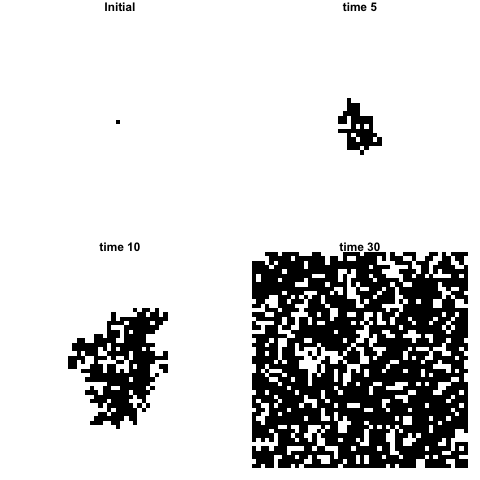
\includegraphics[width=.80\textwidth]{figures/contact_simulation_torus_25.png}
   \caption{Simulation for contact process with $\lambda = 4$ and periodic boundary conditions on $50 \times 50$ grid. The initial configuration is only one node with 1.}
  \label{fig:contact_sim_torus_above_crit.png}
\end{figure}

In Figure \ref{fig:contact_sim_torus_above_crit.png} we show one realization from a simulation of the contact process on $\{0,1\}^{(\Z/50) \times (\Z/50)}$ with $\lambda = 4 \geq \lambda_c(\Z^2)$.
This simulation follows the behavior that the time to extinction is proportional to $\exp(50 \times 50)$.
This is contrasted with Figure \ref{fig:contact_sim_torus_below_crit.png} in which $\lambda = .25$ is smaller than $\lambda_c(\Z^2)$.
The behavior seen on the graph matches shows that the extinction time is proportional to $\log(50 \times 50)$.

\begin{figure}[H]
  \centering
    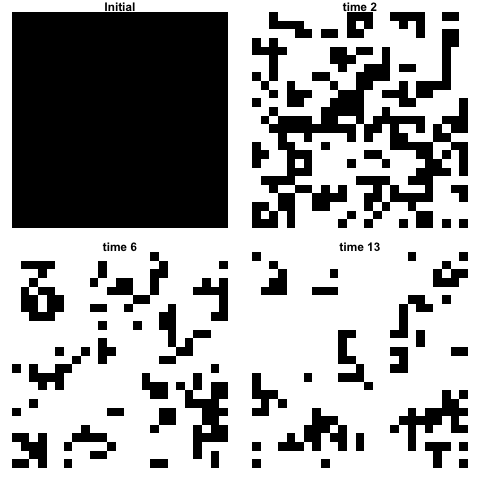
\includegraphics[width=.80\textwidth]{figures/contact_simulation_torus_25_below_crit.png}
   \caption{Simulation for contact process with $\lambda = 0.25$ on $\{0,1\}^{(\Z/50) \times (\Z/50)}$. The initial configuration has all nodes as ones.}
  \label{fig:contact_sim_torus_below_crit.png}
\end{figure}

\section{Contact process on finite graphs}

Now we look at a contact process on a finite graph.
We look at $\tau_{C_2}$ (which depends on $\lambda$), the time until we reach the state zero while keeping the number of nodes fixed as $\lambda$ goes to $\infty$.
% It is known that $\tau_{C_2}$ has a phase-type distribution for a fixed $\lambda$.
As $\lambda \to \infty$ then $\tau_{C_2}$ will converge to infinity in distribution so we will normalize $\tau_{C_2}$ to understand which limiting distribution one can get. This is related to the more general results in \cite{schapira2017} for the limiting distribution of the extinction time of graphs that grow in size rather than $\lambda$.

\begin{theorem}[\cite{schapira2017} Theorem 1.4]
Let $G_n$ be a graph with $n$ vertices and $(G_n)_{n \in \N}$ with $|G_n| \to \infty$ as $n \to \infty$.
Denote $\tau_{G_n}$ as the extinction time of the contact process on graph $G_n$.
For any $\lambda > \lambda_c(\Z)$
$$
\frac{\tau_{G_n}}{E[\tau_{G_n}]} \Rightarrow \exp(1)
$$
\end{theorem}

First we investigate the behavior for a complete graph, in which each node is connected to all other nodes and then we look at the one-dimensional lattice and cycles.


\subsection{Two node contact process \texorpdfstring{$C_2$}{C2}}

The contact process on the finite graph with two nodes and one edge between them has the following transition rates

\begin{align}
    1 &\to 0 \text{ at rate } 1\\
    0 &\to 1 \text{ at rate } \begin{cases}
        \lambda & \text{ if neighbor is 1}\\
        0 & \text{ otherwise}
    \end{cases}
\end{align}

We can express the infinitesimal generator matrix $Q$ matrix as

% Info on blockarray
% https://tex.stackexchange.com/a/59519/41827
$$
Q = \begin{blockarray}{ccccc}
    & (1,1) & (1,0) & (0,1) & (0,0)\\
    \begin{block}{c(cccc)}
        (1,1) & -2 & 1 & 1 & 0\\
        (1,0) & \lambda & - 1 - \lambda & 0 & 1\\
        (0,1) & \lambda & 0 & - 1 - \lambda & 1\\
        (0,0) & 0 & 0 & 0 & 0\\
    \end{block}
\end{blockarray}
$$
Start the process with both nodes at 1.
We can project this continuous-time Markov chain to the number of ones in the process at a given time.
Map $(1,1)$ to 2, $\{(1,0),(0,1)\}$ to a single state 1, and $(0,0)$ to 0.
This new chain is also a Markov chain by Theorem \ref{thm:mc_projection}.

\begin{equation}\label{eq:q_c_2}
Q_{C_2} = \begin{blockarray}{cccc}
    & 2 & 1 & 0\\
    \begin{block}{c(ccc)}
        2 & -2 & 2 & 0\\
        1 & \lambda & - (1 + \lambda) & 1\\
        0 & 0 & 0 & 0\\
    \end{block}
\end{blockarray}
\end{equation}


\begin{figure}[H]
    \centering
   \begin{tikzpicture}[start chain = going right,
   -Triangle, every loop/.append style = {-Triangle}]
   \node[state, on chain]  (2) {2};
   \node[state, on chain]  (1) {1};
   \node[state, on chain]  (0) {0};

   \draw (2) edge[bend left] node[yshift=3mm]{$2$} (1);
   \draw (1) edge[bend left] node[yshift=-3mm]{$\lambda$}(2);
   \draw (1) edge[left] node[xshift=3mm, yshift=-3mm]{$1$} (0);

\end{tikzpicture}
    \caption{Rates for two node projected contact process}
    \label{fig:rates_mc_two_contact}
\end{figure}

\begin{figure}[H]
    \centering
   \begin{tikzpicture}[start chain = going right,
   -Triangle, every loop/.append style = {-Triangle}]
   \node[state, on chain]  (2) {2};
   \node[state, on chain]  (1) {1};
   \node[state, on chain]  (0) {0};

   \draw (2) edge[bend left] node[yshift=3mm]{$1$} (1);
   \draw (1) edge[bend left] node[yshift=-3mm]{$\frac{\lambda}{1 + \lambda}$}(2);
   \draw (1) edge[left] node[xshift=3mm, yshift=-3mm]{$\frac{1}{1 + \lambda}$} (0);

\end{tikzpicture}
    \caption{Embedded Markov chain for two node projected contact process}
    \label{fig:discrete_mc_two_contact}
\end{figure}

Let $\tau_{C_2}$ be the time in which we hit 0.
The waiting time while in state 2 is exponentially distributed random variable $X$ with parameter $- q_{2} = 2$ and similarly the waiting time while in state 1 is exponentially distributed with parameter $- q_{(1,0)} = 1 + \lambda$.

The embedded Markov chain for the process is the discrete-time Markov chain of the jumps in the process.
For example if the original process $(A_t)$ is $A_{0} = 2, A_{.75} = 1, A_{1.2} = 2, \ldots, A_{23.2} = 0$ then the embedded chain $(B_n)$ is $B_{0} = 2, B_1 = 1, B_2 = 2, \ldots, B_n = 0$.
The probability of going from one state to another is shown in Figure \ref{fig:discrete_mc_two_contact}.

Let $N$ be a geometric random variable which denotes the number of times that the process waits at state 1 before moving to the absorbing state 0.
It has a success parameter $\frac{1}{1 + \lambda}$ which represents going to the absorbing state 0.
Also, let $X_1, X_2, \ldots$ be i.i.d random variables with
$X_i \sim \exp(2)$ for the waiting time at state 2 and independent of i.i.d random variables $Y_1, Y_2, \ldots$ with  $Y_i \sim \exp(1 + \lambda)$ for the waiting time at state 1.
The random variable $N$ is independent of both $(X_n)$ and $(Y_n)$ from Theorem \ref{thm:x_N_indep}.

Now we can express $\tau_{C_2}$ as a random sum
$$
\tau_{C_2} = \sum_{i = 1}^N (X_i + Y_i)
$$

\begin{theorem}
$$
E[\tau_{C_2}] = \frac{3}{2} + \frac{\lambda}{2}
$$
and
$$
\Var(\tau_{C_2}) = \frac{\lambda^2 + 6 \lambda + 5}{4}
$$
\end{theorem}

\begin{proof}
$$
P(N = n) = \left(\frac{\lambda}{1 + \lambda} \right)^{n - 1} \frac{1}{1 + \lambda} \quad n = 1,2,\ldots
$$
with
\begin{align*}
    E[N] &= 1 + \lambda\\
    \Var(N) &= \frac{\lambda/(1 + \lambda)}{1/(1 + \lambda)^2} = \lambda (1 + \lambda)
\end{align*}
Also since $(X_n)$ and $(Y_n)$ are independent,

\begin{align*}
    E[X_i + Y_i] &= E[X + Y] = \frac{3 + \lambda}{2(1 + \lambda)}\\
    \Var(X_i + Y_i) &= \Var(X + Y) = \frac{(1 + \lambda)^2 + 4}{4(1 + \lambda)^2}
\end{align*}

Since both $(X_n)$ and $(Y_n)$ are mutually independent of $N$ then by Theorem \eqref{thm:random_sum_ev},
$$
E[\tau_{C_2}] = E\left[ \sum_{i = 1}^N X_i + Y_i \right] = E[X + Y] E[N] = \frac{3 + \lambda}{2(1 + \lambda)} \cdot (1 + \lambda) = \frac{3}{2} + \frac{\lambda}{2}
$$

By Theorem \ref{thm:random_sum_var}
\begin{align*}
    \Var\left( \sum_{i = 1}^N X_i + Y_i \right) &= E[N]\Var(X + Y) + (E[X + Y])^2 \Var(N)\\
    &= (1 + \lambda) \frac{(1 + \lambda)^2 + 4}{4(1 + \lambda)^2} + \frac{(3 + \lambda)^2}{4 (1 + \lambda)^2} \lambda (1 + \lambda)\\
    &= \frac{
        (1 + \lambda)^2 + 4 + (3 + \lambda)^2 \lambda
    }{4(1 + \lambda)}\\
    &= \frac{
    \lambda^3 + 7 \lambda^2 + 11 \lambda + 5
    }{4(1 + \lambda}\\
    &= \frac{\lambda^2 + 6 \lambda + 5}{4}
\end{align*}
\end{proof}

\subsubsection{Phase-type distribution}

The time to absorption $\tau_{C_2}$ has a phase-type distribution.
We can decompose $Q_{C_2}$, Equation \eqref{eq:q_c_2}, as
% $$
% Q_{C_2} = \begin{blockarray}{cccc}
%     & 2 & 1 & 0\\
%     \cline{2-4}
%     \begin{block}{c|cc|c|}
%         2 & -2 & 2 & 0\\
%         1 & \lambda & - (1 + \lambda) & 1\\
%         \cline{2-3}
%     \end{block}
%     \begin{block}{c|ccc|}
%         0 & 0 & 0 & 0\\
%     \end{block}
% \end{blockarray}
% $$
\begin{align*}
    \mathbf{S} &= \begin{pmatrix}
        -2 & 2\\
        \lambda & - (1 + \lambda)
    \end{pmatrix}\\
    \mathbf{S}_0 &= \begin{pmatrix}
        0\\
        1
    \end{pmatrix}\\
    \boldsymbol{\alpha} &= \begin{pmatrix}
    1 & 0
    \end{pmatrix}
\end{align*}

To compute the matrix exponential $\exp(x S)$ we first compute the eigenvalues of $S$.
Solving $\det(S - m I) = 0$ for $m$,
\begin{align*}
    \det(S - m I) &= \det\left(\begin{bmatrix}
        -2 - m & 2\\
        \lambda & - 1 - \lambda - m
    \end{bmatrix} \right)\\
    &= (2 + m) (1 + \lambda + m) - 2 \lambda\\
    &= 2 + (3 + \lambda) m + m^2
\end{align*}
Solving the equation $2 + (3 + \lambda) m + m^2 = 0$ for $m$ we get roots (eigenvalues)
\begin{align*}
    m_1 &= \frac{1}{2}(-3 - \lambda + \sqrt{\lambda^2 + 6 \lambda + 1})\\
    m_2 &= \frac{1}{2}(-3 - \lambda - \sqrt{\lambda^2 + 6 \lambda + 1})
\end{align*}
So $\lambda_1 = x m_1$, $\lambda_2 = x m_2$ are the eigenvalues for $x S$.
Denote
$$
\Lambda = \operatorname{diag}(\lambda_1, \lambda_2)
$$
and
$$
C = \sqrt{\lambda^2 + 6 \lambda + 1}
$$
Then solving $(S - m I) \mathbf{v} = 0$ for $m_1, m_2$, we get eigenvectors
\begin{align*}
    v_1 &= \left( \frac{-1 + \lambda - C}{2\lambda}, 1 \right)\\
    v_2 &= \left( \frac{-1 + \lambda + C}{2\lambda}, 1 \right)
\end{align*}
Let
$$
U = \begin{bmatrix}
    \frac{-1 + \lambda - C}{2\lambda} & \frac{-1 + \lambda + C}{2\lambda}\\
    1 & 1
\end{bmatrix}
$$
hence
$$
\det(U) = - \frac{C}{\lambda}
$$
It follows that
\begin{align*}
    U^{-1} &= - \frac{\lambda}{C} \begin{bmatrix}
    1 & \frac{1 - \lambda - C}{2\lambda}\\
    -1 & \frac{-1 + \lambda - C}{2\lambda}
    \end{bmatrix}\\
    &= \frac{1}{2C} \begin{bmatrix}
    -2\lambda & -1 + \lambda + C\\
    2\lambda & 1 - \lambda + C
    \end{bmatrix}
\end{align*}

% Now by Theorem \ref{thm:eigen_matrix_exp}, we can compute $\exp(xS)$ as
% \begin{align*}
% \exp(xS) &= T \begin{bmatrix}
%     \exp(\frac{1}{2}(-3 - \lambda + C)) & 0\\
%     0 & \exp(\frac{1}{2}(-3 - \lambda - C))
% \end{bmatrix} T^{-1}\\
% &= - \frac{1}{2 C} T \begin{bmatrix}
%     \exp(\frac{-3 - \lambda + C}{2}) & \exp(\frac{-3 - \lambda + C}{2}) \frac{1 - \lambda - C}{2\lambda} \\
%     - \exp(\frac{-3 - \lambda - C}{2}) & \exp(\frac{1}{2}(-3 - \lambda - C)) \frac{-1 + \lambda - C}{2\lambda}
% \end{bmatrix}
% \end{align*}

The density of $\tau_{C_2}$ is defined as
\begin{align*}
 f(x; \lambda) &= \boldsymbol{\alpha} \exp(x \mathbf{S}) \mathbf{S}_0 \nonumber\\
 &= (1, 0) \exp(\mathbf{S} x) (0,1)^T \\
 &= (1, 0) U \exp(\Lambda) U^{-1} (0,1)^T
\end{align*}
Where
\begin{align*}
    (1,0) U &= (1,0) \begin{bmatrix}
    \frac{-1 + \lambda - C}{2\lambda} & \frac{-1 + \lambda + C}{2\lambda}\\
    1 & 1
\end{bmatrix}\\
    &= \begin{bmatrix}
    \frac{-1 + \lambda - C}{2\lambda} & \frac{-1 + \lambda + C}{2\lambda}
    \end{bmatrix}
\end{align*}
and
\begin{align*}
    U^{-1} (0,1)^T &= \frac{1}{2C} \begin{bmatrix}
    -2\lambda & -1 + \lambda + C\\
    2\lambda & 1 - \lambda + C
    \end{bmatrix} (0,1)^T\\
    &= \frac{1}{2C} \begin{bmatrix}
    -1 + \lambda + C\\
    1 - \lambda + C
    \end{bmatrix}
\end{align*}

Thus
\begin{align*}
     f(x; \lambda) &= (1, 0) U \exp(\Lambda) U^{-1} (0,1)^T\\
     &= \frac{1}{2C} \begin{bmatrix}
    \frac{-1 + \lambda - C}{2\lambda} & \frac{-1 + \lambda + C}{2\lambda}
    \end{bmatrix} \exp(\Lambda)  \begin{bmatrix}
    -1 + \lambda + C\\
    1 - \lambda + C
    \end{bmatrix}\\
    &= \frac{1}{2C} \left( 4 \exp\left(\frac{1}{2}(-3 - \lambda + C) x\right) - 4 \exp\left(\frac{1}{2}(-3 - \lambda - C) x\right) \right)\\
    &= \frac{2}{C} \left( \exp\left(\frac{1}{2}(-3 - \lambda + C) x\right) - \exp\left(\frac{1}{2}(-3 - \lambda - C) x\right) \right)\\
\end{align*}
Note that the left exponential and right exponential differ only by sign on the term $C$.
Finally plugging back in $C$ we get
\begin{equation} \label{eq:t_density}
      f(x; \lambda) = \frac{2 \exp\left(\frac{1}{2}(-3 - \lambda + \sqrt{\lambda^2 + 6 \lambda + 1}) x\right)}{\sqrt{\lambda^2 + 6 \lambda + 1}}  - \frac{2 \exp\left(\frac{1}{2}(-3 - \lambda - \sqrt{\lambda^2 + 6 \lambda + 1}) x\right)}{\sqrt{\lambda^2 + 6 \lambda + 1}}
\end{equation}

% \begin{align}
% f(x; \lambda) &= \boldsymbol{\alpha} \exp(x \mathbf{S}) \mathbf{S}_0 \nonumber\\
% &= (1, 0) \exp(\mathbf{S} x) (0,1)^T \nonumber\\
% &= (1, 0) T \begin{bmatrix}
%     \exp(\frac{1}{2}(-3 - \lambda + \sqrt{\lambda^2 + 6 \lambda + 1})) & 0\\
%     0 & \exp(\frac{1}{2}(-3 - \lambda - \sqrt{\lambda^2 + 6 \lambda + 1}))
% \end{bmatrix} T^{-1}
% (0,1)^T \nonumber\\
% &=
% \left(\frac{-1 + \lambda - \sqrt{\lambda^2 + 6 \lambda + 1}}{2\lambda}, 1\right) \nonumber \\
% &\quad\quad \begin{bmatrix}
%     \exp(\frac{1}{2}(-3 - \lambda + \sqrt{\lambda^2 + 6 \lambda + 1})) & 0\\
%     0 & \exp(\frac{1}{2}(-3 - \lambda - \sqrt{\lambda^2 + 6 \lambda + 1}))
% \end{bmatrix} \nonumber\\
% &\quad\quad  \begin{bmatrix}
%     \frac{1 - \lambda - \sqrt{\lambda^2 + 6 \lambda + 1}}{2\lambda}\\
%     \frac{-1 + \lambda - \sqrt{\lambda^2 + 6 \lambda + 1}}{2\lambda}
% \end{bmatrix} \nonumber
% \end{align}

% MatrixExp[{{-2 x, 2 x}, {\[Lambda] x, -((1 + \[Lambda]) x)}}] // TeXForm

% Using Wolfram Language we can compute the matrix exponential which is complicated even in this simple case. Let $A = \exp(Sx)$.

% \begin{align*}
% A_{11} &= \frac{\left(C+\lambda -1\right) e^{\frac{1}{2}
%   \left(C-\lambda -3\right) x}}{2 C}\\
%   &\quad\quad- \frac{\left(-C+\lambda -1\right)
%   e^{\frac{1}{2} \left(-C-\lambda -3\right) x}}{2
%   C}\\
%   A_{12} &= \frac{2 e^{\frac{1}{2} \left(C-\lambda -3\right) x}}{C}-\frac{2
%   e^{\frac{1}{2} \left(-C-\lambda -3\right)
%   x}}{C}\\
%   A_{21} &= \frac{\lambda  e^{\frac{1}{2} \left(C-\lambda -3\right)
%   x}}{C}-\frac{\lambda  e^{\frac{1}{2}
%   \left(-C-\lambda -3\right) x}}{C}\\
%   A_{22} &= \frac{\left(C-\lambda +1\right)
%   e^{\frac{1}{2} \left(C-\lambda -3\right) x}}{2
%   C}\\
%   &\quad\quad-\frac{\left(-C-\lambda +1\right) e^{\frac{1}{2} \left(-C-\lambda
%   -3\right) x}}{2 C}
% \end{align*}

% Then the density of $\tau_{C_2}$ is defined as
% \begin{align}
% f(x; \lambda) &= \boldsymbol{\alpha} \exp(x \mathbf{S}) \mathbf{S}_0 \nonumber\\
% &= (1, 0) \exp(\mathbf{S} x) (0,1)^T \nonumber\\
% &= \exp(\mathbf{S} x)_{12} \nonumber\\
% &= \frac{2 e^{\frac{1}{2} \left(\sqrt{\lambda ^2+6
%   \lambda +1}-\lambda -3\right) x}}{C}-\frac{2
%   e^{\frac{1}{2} \left(-C-\lambda -3\right)
%   x}}{C} \label{eq:t_density}
% \end{align}

\begin{figure}[H]
  \centering
    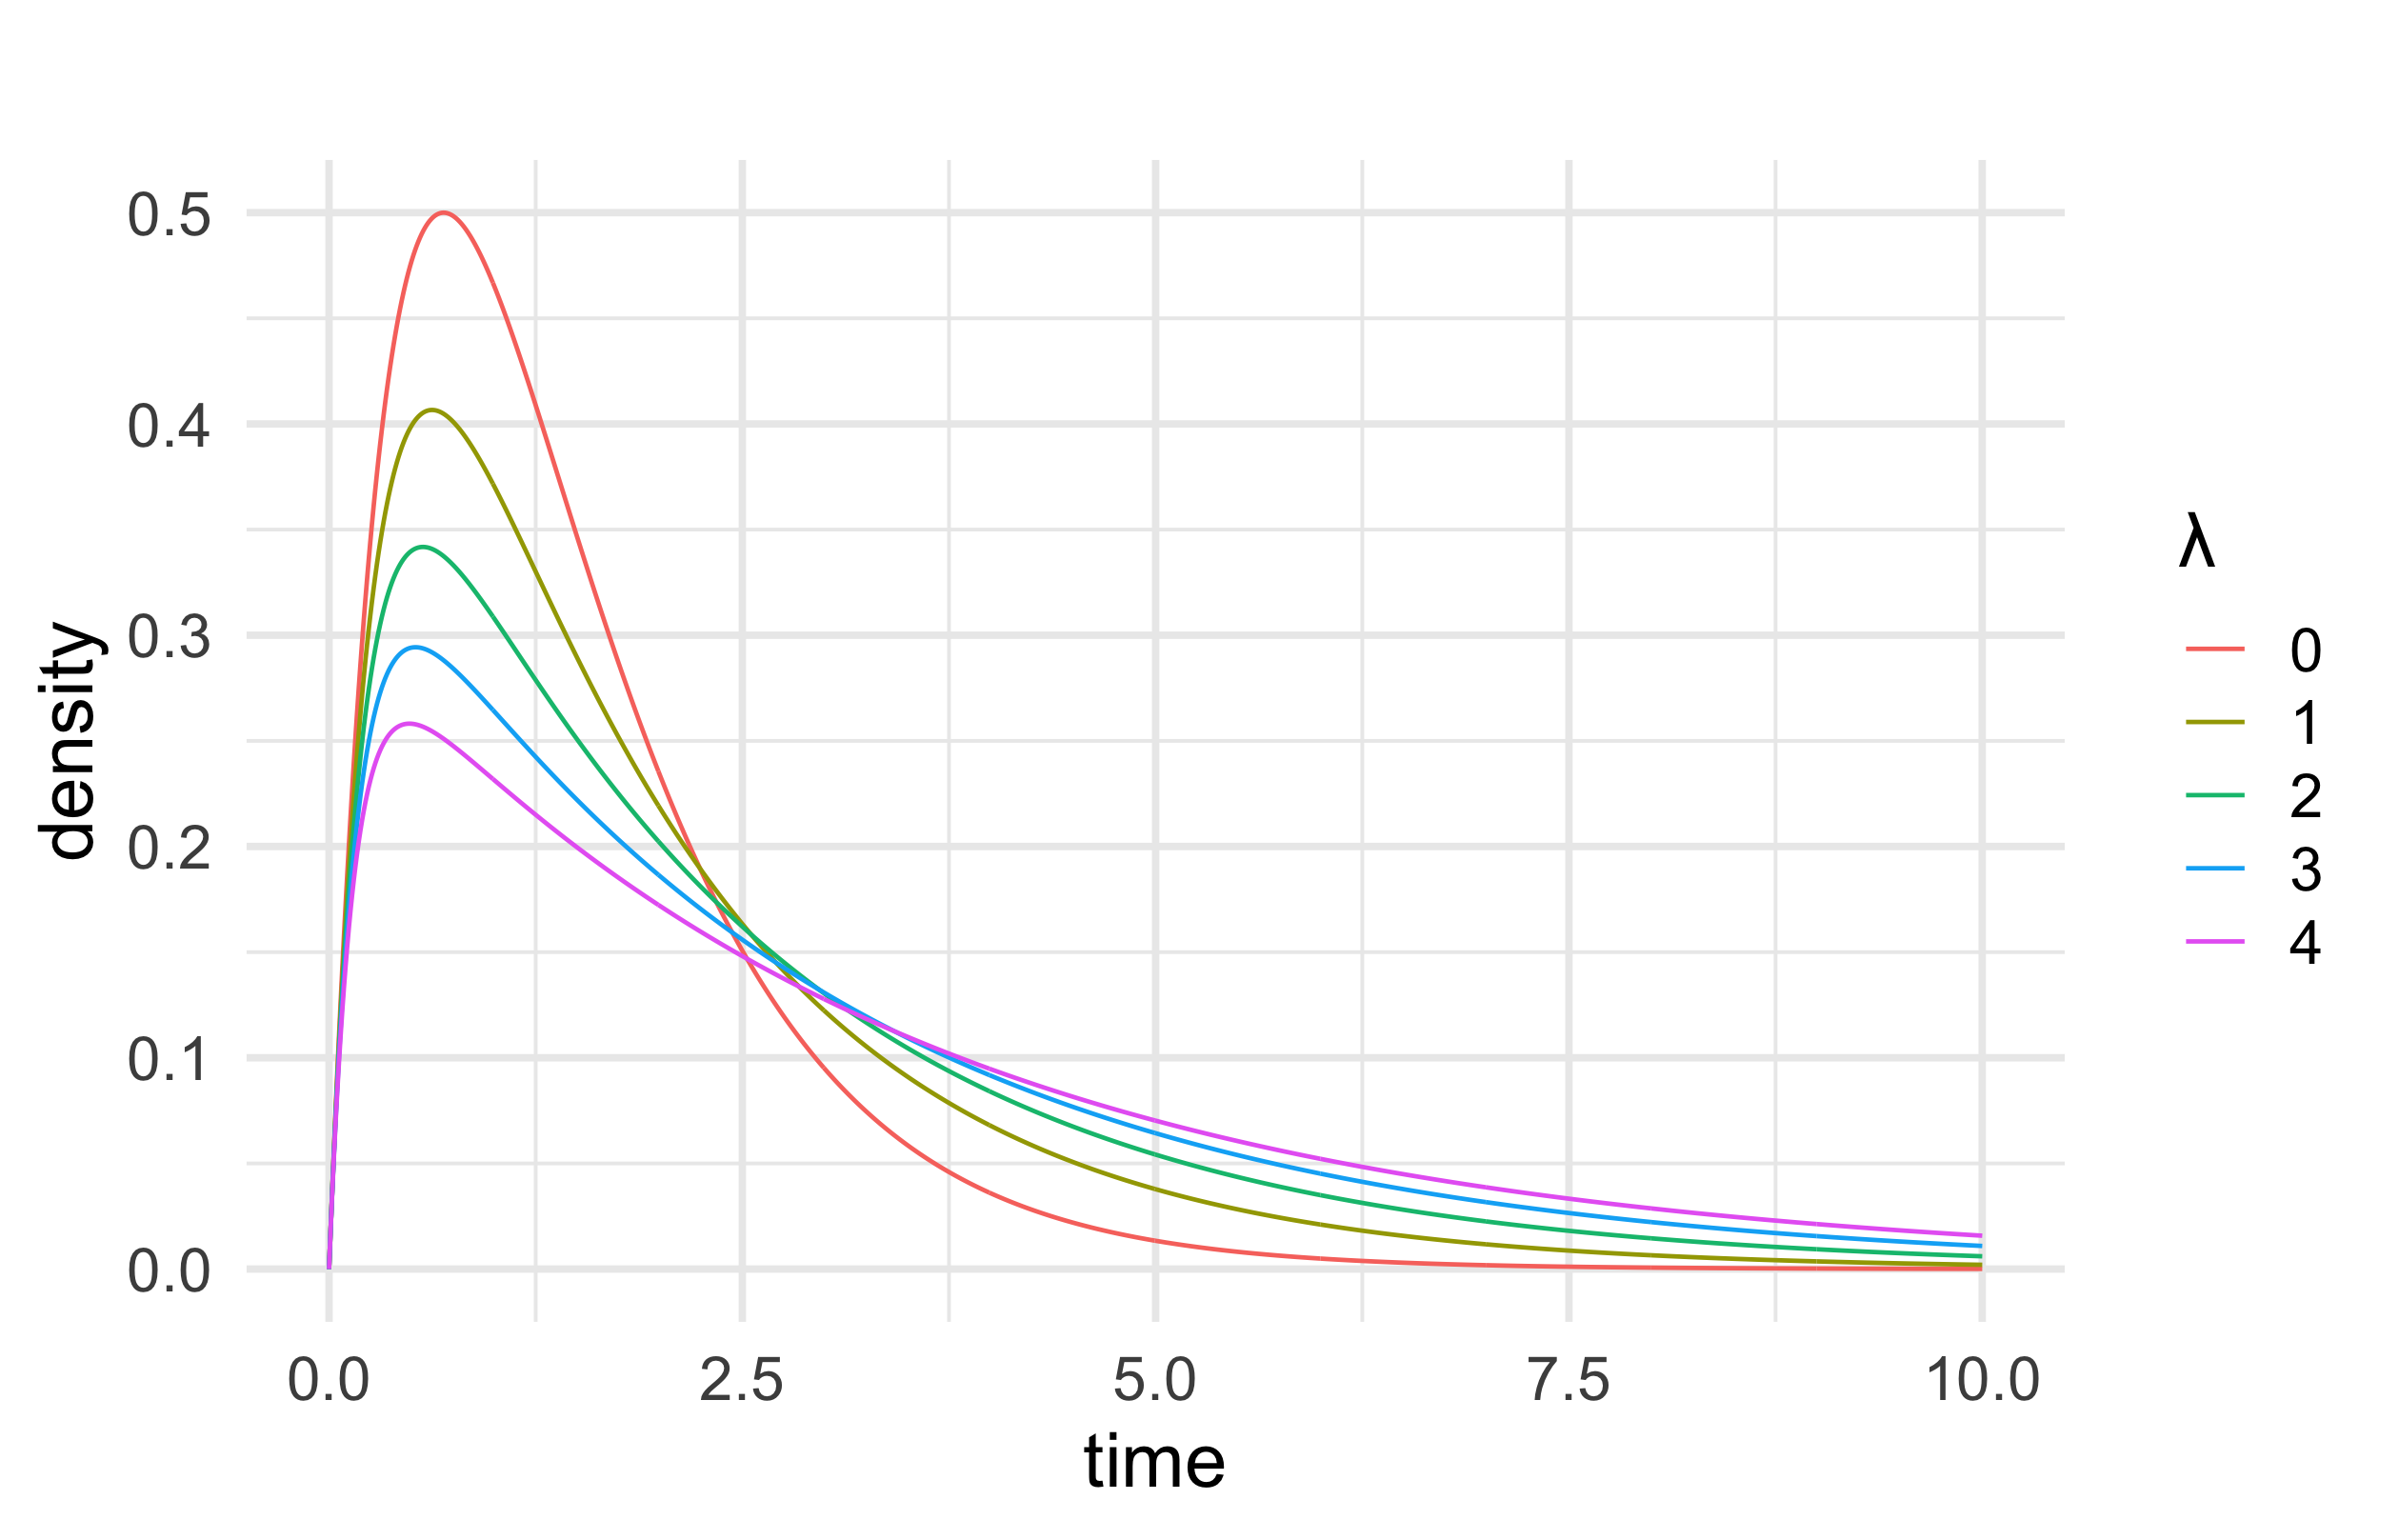
\includegraphics[width=.80\textwidth]{figures/complete_2_contact_phase_densities.png}
   \caption{Density functions for $\tau_{C_2}$ for $\lambda = 1, 2, 3, 4$ on the contact process with two nodes}
  \label{fig:contact_2_phase_densities}
\end{figure}

In Figure \ref{fig:contact_2_phase_densities} we plot the density from Equation \ref{eq:t_density} for $\lambda = 1, 2, 3, 4$.
It is clear that as $\lambda \to \infty$ then $\tau_{C_2}$ approaches infinity in distribution.
For all of the more complex models we will use numerical methods for approximating the phase-type distribution rather than the symbolic algebra method.
We sample and simulate from the phase-type distributions using the R package from \cite{actuar2008}.

\subsubsection{Limiting Distribution}

\begin{theorem}\label{thm:exp_limiting_dist}
Assume that $X$ is exponentially distributed with parameter $\alpha(n)$.
If $\alpha(n) \to \infty$ as $n \to \infty$ then $X$ approaches 0 in distribution.
\end{theorem}

\begin{proof}
Assume $X$ is exponentially distributed with parameter $\alpha(n)$.
Note that 0 has a CDF of
$$
F_0(x) = \begin{cases}
    1 & x \geq 0\\
    0 & x < 0
\end{cases}
$$
Then $X$ has a CDF, with $x \in [0, \infty)$
$$
F_X(x) = 1 - \exp(-\alpha(n) x) \to 1 \quad \text{ as } n \to \infty
$$
So
$$
\exp(\alpha(n)) \Rightarrow 0 \quad \text{ as } n \to \infty
$$
\end{proof}

\begin{theorem}
Let $\tau_{C_2}$ be the time in which we hit $(0,0)$.
Then $\frac{2}{1 + \lambda} \tau_{C_2}$ approaches an exponential distribution with rate 1 in distribution as $\lambda \to \infty$.
\end{theorem}

\begin{proof}
Let $X_1, X_2, \ldots$ be i.i.d random variables with
$X_i \sim \exp(2)$ and independent of i.i.d random variables $Y_1, Y_2, \ldots$ with  $Y_i \sim \exp(1 + \lambda)$ and
$N$ geometrically distributed (supported on $\{1,2,\ldots\}$) with parameter $\frac{1}{1 + \lambda}$, independent of $(X_n)$ and $(Y_n)$.

$\tau_{C_2}$ is expressed as a random sum
$$
\tau_{C_2} = \sum_{i = 1}^N (X_i + Y_i)
$$

By Theorem \ref{thm:geom_sum_exp}, we have that
\begin{align*}
    \sum_{i = 1}^N X_i &\sim \exp\left( \frac{2}{1 + \lambda} \right)\\
    \sum_{i = 1}^N Y_i &\sim \exp( 1 )
\end{align*}

Using the scaling property of exponential random variables (Theorem \ref{thm:exp_scaling}) we have that
\begin{align*}
    \frac{2}{1 + \lambda}\sum_{i = 1}^N X_i &\sim \exp( 1 )\\
    \frac{2}{1 + \lambda}\sum_{i = 1}^N Y_i &\sim \exp \left( \frac{1 + \lambda}{2} \right)
\end{align*}

Since $(1 + \lambda)/2 \to \infty$ as $\lambda \to \infty$ then we have a limit of two sequences of random variables, one of which converges in distribution to a constant. So by Theorem \ref{thm:exp_limiting_dist} we can conclude that 
$$
\frac{2}{1 + \lambda}\sum_{i = 1}^N Y_i \Rightarrow 0
$$
Then by Theorem \ref{thm:conv_together_lemma}, we have that
$$
\frac{2}{1 + \lambda} \tau_{C_2} \Rightarrow \exp(1)
$$
\end{proof}

\subsection{Three node contact process \texorpdfstring{$C_3$}{C3}}
Now we look at the three node contact process on a complete graph.
Again we project the states to the number of ones in the process which will be a Markov chain by Theorem \ref{thm:mc_projection}, as shown in Figure \ref{fig:mc_three_contact}.

% {{-3x, 3x, 0}, {2\[Lambda] x, -(2 + 2 \[Lambda]) x, 2x}, {0, 2\[Lambda]x, -(1 + 2\[Lambda])x}}
% Computing the matrix exponential is crazy. Better to leave numeric.
\begin{equation}
Q_{C_3} = \begin{blockarray}{ccccc}
    & 3 & 2 & 1 & 0\\
    \begin{block}{c|cccc}
    \cline{2-5}
        3 & -3 & 3 & 0 & 0 \\
        2 & 2\lambda & -(2 + 2 \lambda) &
        2 & 0\\
        1 & 0 & 2\lambda & -(1 + 2\lambda) & 1\\
    0 & 0 & 0 & 0 & 0\\
    \end{block}
\end{blockarray}
\end{equation}

Now let $N_1, N_2, N_3$ be the number of visits to states 1, 2, and 3, respectively.
Let $X_i^{(1)} \sim \exp(1 + 2\lambda)$ be i.i.d random variables, $X_i^{(2)} \sim \exp(2 + 2\lambda)$ i.i.d and $X_i^{(3)} \sim \exp(3)$ i.i.d.
Note that $N_1, N_2, N_3$ are not independent of each other, but for each $i$ each state is independent of the waiting times at the state.
We can again represent $\tau_{C_3}$ as a random sum

\begin{figure}[H]
    \centering
   \begin{tikzpicture}[start chain = going right,
   -Triangle, every loop/.append style = {-Triangle}]
   \node[state, on chain]  (3) {3};
   \node[state, on chain]  (2) {2};
   \node[state, on chain]  (1) {1};
   \node[state, on chain]  (0) {0};

   \draw (3) edge[bend left] node[yshift=3mm]{$3$} (2);
   \draw (2) edge[bend left] node[yshift=-3mm]{$2\lambda$}(3);
   %
   \draw (2) edge[bend left] node[yshift=3mm]{$2$} (1);
   \draw (1) edge[bend left] node[yshift=-3mm]{$2\lambda$}(2);
   %
   \draw (1) edge[left] node[xshift=3mm, yshift=-3mm]{$1$} (0);

\end{tikzpicture}
    \caption{Projected Markov chain rates of number of ones for three node contact process}
    \label{fig:mc_three_contact}
\end{figure}

\begin{equation}
    \tau_{C_3} = \sum_{i = 1}^{N_3} X_i^{(3)} + \sum_{i = 1}^{N_2} X_i^{(2)} + \sum_{i = 1}^{N_1} X_i^{(1)}
\end{equation}

Then the discrete time Markov chain for this process can be expressed in canonical form as
$$
P_{C_3} = \begin{blockarray}{ccccc}
    & 3 & 2 & 1 & 0\\
    \begin{block}{c|ccc|c}
    \cline{2-5}
        3 & 0 & 1 & 0 & 0 \\
        2 & \frac{\lambda}{1 + \lambda} & 0 &
        \frac{1}{1 + \lambda} & 0\\
        1 & 0 & \frac{2\lambda}{1 + 2 \lambda} & 0 & \frac{1}{1 + 2\lambda}\\
    \cline{2-4}
    \end{block}
    \begin{block}{c|cccc}
    0 & 0 & 0 & 0 & 1\\
    \end{block}
\end{blockarray}
$$

\begin{figure}[H]
    \centering
   \begin{tikzpicture}[start chain = going right,
   -Triangle, every loop/.append style = {-Triangle}]
   \node[state, on chain]  (3) {3};
   \node[state, on chain]  (2) {2};
   \node[state, on chain]  (1) {1};
   \node[state, on chain]  (0) {0};

   \draw (3) edge[bend left] node[yshift=3mm]{$1$} (2);
   \draw (2) edge[bend left] node[yshift=-3mm]{$\frac{ \lambda}{1 + \lambda}$}(3);
   %
   \draw (2) edge[bend left] node[yshift=3mm]{$\frac{1}{1 + \lambda}$} (1);
   \draw (1) edge[bend left] node[yshift=-3mm]{$\frac{2\lambda}{1 + 2 \lambda}$}(2);
   %
   \draw (1) edge[left] node[xshift=3mm, yshift=-3mm]{$\frac{1}{1 + 2\lambda}$} (0);

\end{tikzpicture}
    \caption{Embedded discrete Markov chain for projection to number of ones for three node contact process}
    \label{fig:discrete_mc_three_contact}
\end{figure}

Since the discrete Markov chain is absorbing, with 0 as an absorbing state, we can compute the expected number of visits to each state using the fundamental matrix.

% Wolfram:
% B = {{1, -1, 0},{-x/(2 + x), 1, -2/(2 + x)},{0, -2x/(1 + 2x), 1}}
% inverse of {{1, -1, 0},{-x/(1 + x), 1, -1/(1 + x)},{0, -2x/(1 + 2x), 1}}

Let $B$ be the transition matrix for the transient states 3, 2, and 1.
$$
B_{C_3} = \begin{blockarray}{cccc}
    & 3 & 2 & 1\\
    \begin{block}{c|ccc}
    \cline{2-4}
        3 & 0 & 1 & 0\\
        2 & \frac{\lambda}{1 + \lambda} & 0 &
        \frac{1}{1 + \lambda}\\
        1 & 0 & \frac{2\lambda}{1 + 2 \lambda} & 0\\
    \end{block}
    \end{blockarray}
$$
Then by Theorem \ref{thm:fund_exp} the expected number of times that the contact process has a given state is given by,
$$
    I + B_{C_3} + B_{C_3}^2 + \cdots = (I - B_{C_3})^{-1} = \begin{blockarray}{cccc}
    & 3 & 2 & 1\\
    \begin{block}{c|ccc}
    \cline{2-4}
    3 & 2 \lambda^2 + \lambda + 1 & (\lambda + 1) (2 \lambda + 1) &  2 \lambda + 1\\
    2 & \lambda (2 \lambda + 1) & (\lambda + 1)(2 \lambda + 1) & 2 \lambda + 1\\
    1 & 2 \lambda^2 & 2 \lambda ( \lambda + 1) &  2\lambda + 1\\
    \end{block}
    \end{blockarray}
$$
The first row corresponds to the expected number of visits to each state given that we started in state 3 (all the nodes initialized to 1).
Thus,
\begin{align*}
    E[N_1] &= 2 \lambda + 1\\
    E[N_2] &= (\lambda + 1) (2 \lambda + 1) = 2\lambda^2 + 3 \lambda + 1\\
    E[N_3] &=  2 \lambda^2 + \lambda + 1
\end{align*}

Since $N_1, N_2, N_3$ are all geometrically distributed and are completely determined by the mean we can conclude that
\begin{align*}
    N_1 &\sim  \text{Geom}\left(\frac{1}{2 \lambda + 1} \right)\\
    N_2 &\sim \text{Geom}\left(\frac{1}{2\lambda^2 + 3 \lambda + 1} \right)\\
    N_3 &\sim  \text{Geom}\left(\frac{1}{2 \lambda^2 + \lambda + 1}\right)
\end{align*}

It then follow that
\begin{align*}
        E[\tau_{C_3}] &= E[N_3] E[X_i^{(3)}] + E[N_2] E[X_i^{(2)}] + E[N_1] E[X_i^{(1)}]\\
        &= \frac{\lambda^2 + \lambda + 1}{3} + \frac{(\lambda + 1)(2 \lambda + 1)}{2 (\lambda + 1)} + \frac{1 + 2\lambda}{1 + 2 \lambda}\\
        &= \frac{1}{6}(4 \lambda^2 + 8 \lambda + 11)
\end{align*}

\subsubsection{Phase-type Distribution}

The exact distribution of $\tau_{C_3}$ for a fixed $\lambda$ is computed numerically.
We plot the density functions for $\tau_{C_3}$ for $\lambda = 1, 2, 3, 4$ on the complete three node contact process.

\begin{figure}[H]
  \centering
    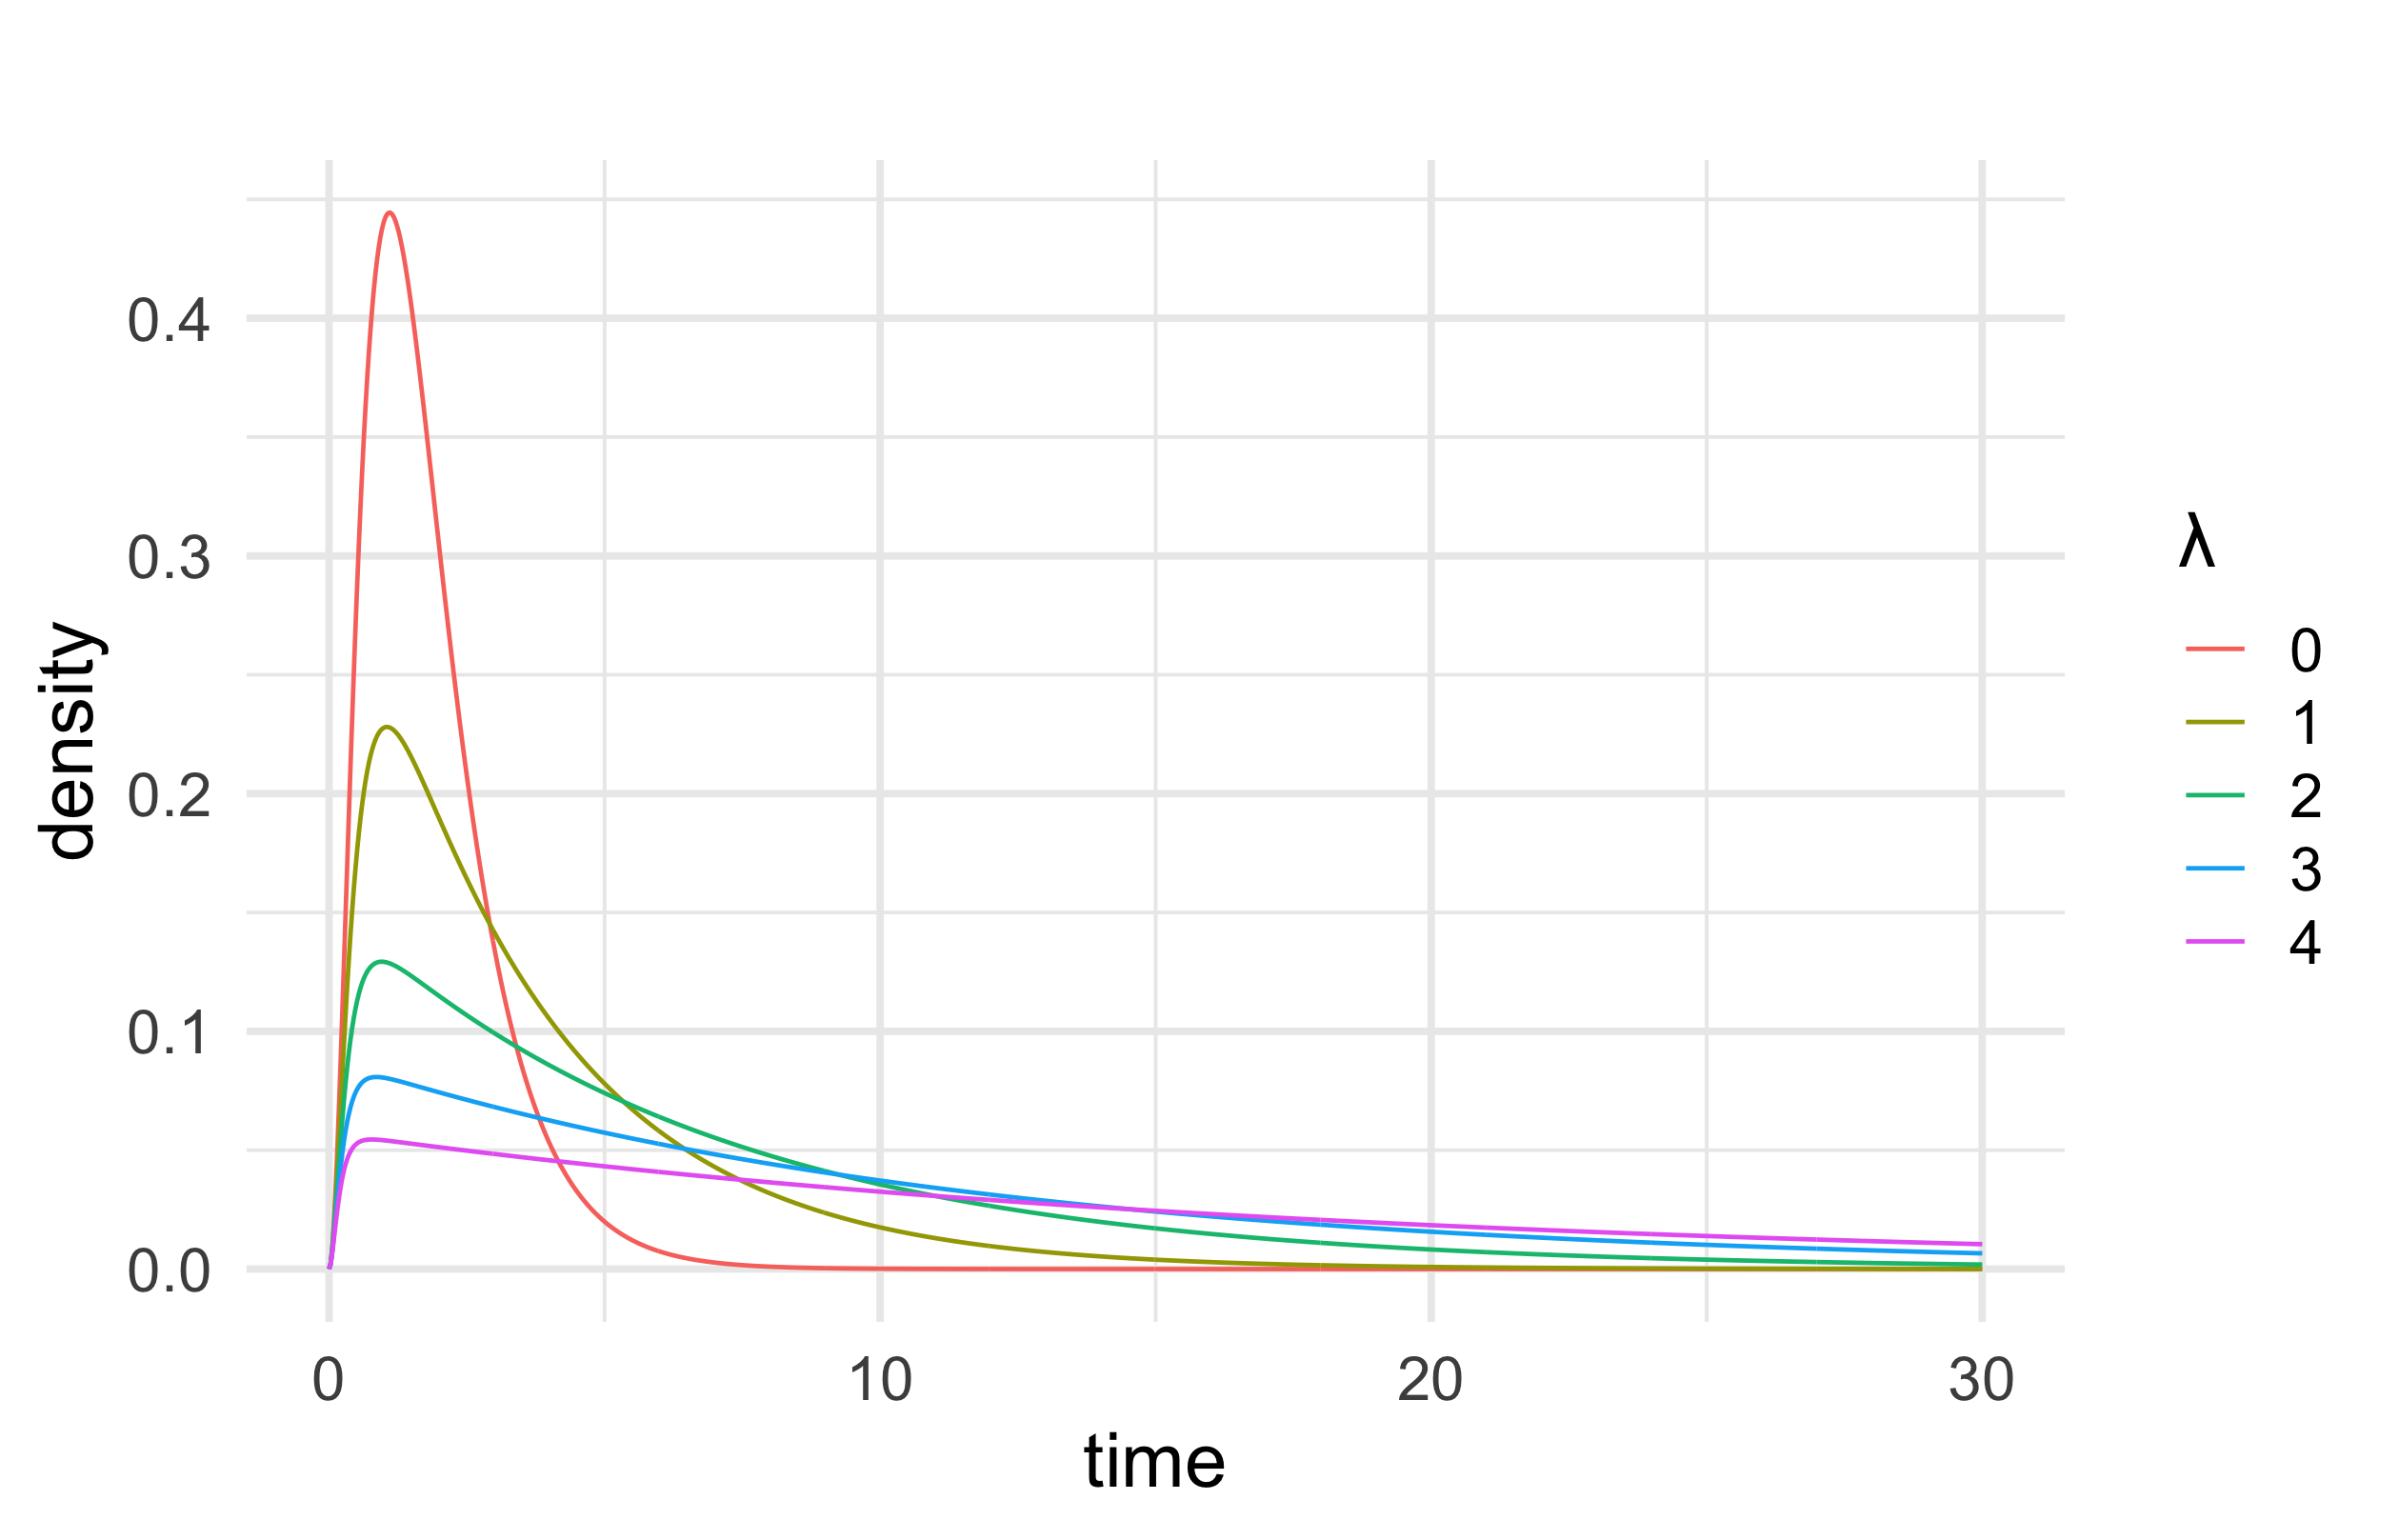
\includegraphics[width=.80\textwidth]{figures/complete_3_contact_phase_densities.png}
   \caption{Density functions for $\tau_{C_3}$ for $\lambda = 1, 2, 3, 4$ on the complete three node contact process}
  \label{fig:contact_3_phase_densities}
\end{figure}

\subsubsection{Limiting Distribution}

\begin{theorem}
Let $\tau_{C_3}$ be the time in which we hit 0 in the three node complete contact process.
Then $\frac{3}{2 \lambda^2 + \lambda + 1} \tau_{C_3}$ converges in distribution to an exponential distribution with rate 1.
\end{theorem}

\begin{proof}
By Theorem \eqref{thm:geom_sum_exp}, we have that
\begin{align*}
    \sum_{i = 1}^{N_3} X_i^{(3)} &\sim \exp\left(
        \frac{3}{2\lambda^2 + \lambda + 1}
        \right) \\
    \sum_{i = 1}^{N_2} X_i^{(2)} &\sim \exp\left(
        \frac{2 + 2\lambda}{2 \lambda^2 + 3\lambda + 1}
    \right)\\
    \sum_{i = 1}^{N_1} X_i^{(1)} &\sim \exp\left(\frac{1 + 2\lambda}{1 + 2\lambda}\right)
\end{align*}

Multiplying $\tau_{C_3}$ by $\frac{3}{2 \lambda^2 + \lambda + 1}$ and using Theorem \eqref{thm:exp_scaling}, we get
\begin{align*}
    \frac{3}{2 \lambda^2 + \lambda + 1} \sum_{i = 1}^{N_3} X_i^{(3)} &\sim \exp\left(
        1
        \right)\\
    \frac{3}{2 \lambda^2 + \lambda + 1} \sum_{i = 1}^{N_2} X_i^{(2)} &\sim \exp\left(
        \frac{(2 + 2\lambda)(2 \lambda^2 + \lambda + 1)}{3 (2 \lambda^2 + 3\lambda + 1)}
    \right)\\
    \frac{3}{2 \lambda^2 + \lambda + 1} \sum_{i = 1}^{N_1} X_i^{(11)} &\sim \exp\left(
        \frac{2 \lambda^2 + \lambda + 1}{3}
    \right)
\end{align*}    
Since
\begin{align*}
    \frac{(2 + 2\lambda)(2 \lambda^2 + \lambda + 1)}{3 (2 \lambda^2 + 3\lambda + 1)} &= \frac{4\lambda^3 + 6 \lambda^2 + 4 \lambda + 2}{6\lambda^2 + 9\lambda + 3}
    \to \infty \quad \text{as } \lambda \to \infty
\end{align*}
It follows that
$$
    \frac{3}{2 \lambda^2 + \lambda + 1} \sum_{i = 1}^{N_2} X_i^{(2)} \sim \exp\left(
        \frac{4\lambda^3 + 6 \lambda^2 + 4 \lambda + 2}{6\lambda^2 + 9\lambda + 3}
    \right) \Rightarrow 0 \quad \text{as } \lambda \to \infty
$$
So
$$
\frac{3}{2 \lambda^2 + \lambda + 1} \sum_{i = 1}^{N_2} X_i^{(2)} \Rightarrow 0 \quad \text{as } \lambda \to \infty
$$
Similarly we have that
$$
\frac{3}{2 \lambda^2 + \lambda + 1} \sum_{i = 1}^{N_1} X_i^{(1)}
$$

Since we have a sum of three random variables, two of which approach 0 in distribution, we can use Theorem \ref{thm:conv_together_lemma} to conclude that  $\frac{3}{2 \lambda^2 + \lambda + 1} \tau_{C_3}$ converges in distribution to an exponential distribution with rate 1.
\end{proof}

\subsection{N node complete graph contact process \texorpdfstring{$C_n$}{Cn}}

\begin{figure}[H]
    \centering
   \begin{tikzpicture}[
   start chain = going right,
   -Triangle,
   every loop/.append style = {-Triangle}]
   \node[state, on chain]  (n) {n};
   \node[state, on chain]  (n1) {n - 1};
   \node[state, on chain]  (n2) {n - 2};
   \node[state without output/.append style={draw=none}, on chain]  (dots1) {...};
   \node[state, on chain]  (2) {2};
   \node[state, on chain]  (1) {1};
   \node[state, on chain]  (0) {0};

   \draw (n) edge[bend left] node[yshift=3mm]{$n$} (n1);
   \draw (n1) edge[bend left] node[yshift=-3mm]{$1 (n - 1) \lambda$}(n);

   \draw (n1) edge[bend left] node[yshift=3mm]{$n-1$} (n2);
   \draw (n2) edge[bend left] node[yshift=-3mm]{$2 (n - 2)\lambda$}(n1);

   \draw (n2) edge[left] node[xshift=3mm, yshift=-3mm]{} (dots1);

   \draw (dots1) edge[left] node[xshift=3mm, yshift=-3mm]{} (2);

  \draw (2) edge[bend left] node[yshift=3mm]{$2$} (1);
   \draw (1) edge[bend left] node[yshift=-3mm]{$(n - 1)1 \lambda$}(2);

  \draw (1) edge[left] node[yshift=3mm]{$1$} (0);
\end{tikzpicture}
    \caption{Transition rates for N node complete contact process}
    \label{fig:complete_contact_n_node_rates}
\end{figure}

In Figure \ref{fig:complete_contact_n_node_rates}, we show the transition rates for between the states of the contact process on the complete graph.
Note that for $i \in \{1,\ldots, n - 1\} $ nodes that have a state of one, we have that the rate of going to $i + 1$ nodes is one of the $n - i$ nodes turning to one, each at a rate of $\lambda i$.
Thus, a total rate of $i (n - i) \lambda$.
The rate of going state with $i - 1$ ones is $i$ since we have $i$ nodes that have a potential to switch to zero, each with a rate of one.

\begin{align*}
    i \to i - 1 &= \begin{cases}
        0 & i \in 0\\
        i & i \in \{1,\ldots, n\}
    \end{cases}\\
    i \to i + 1 &= \begin{cases}
        0 & i = i \in \{0, n\}\\
        i(n - i) \lambda & i \in \{1,\ldots, n-1\}
    \end{cases}
\end{align*}

\begin{lemma}[This is a generalization of Lemma \ref{lem:rw_hit_zero}]\label{lem:rw_p_hit_zero}
Assume that we have a random walk with $p \in (0, 1)$, $p \not = 1/2$, on $\{0,1,\ldots, n\}$ with transition probabilities 
\begin{align*}
    i \to i - 1 &= \begin{cases}
        1 & i = n\\
        1 - p & i \in \{1,\ldots, n\}
    \end{cases}\\
    i \to i + 1 &= \begin{cases}
        0 & i = n\\
        p & i \in \{1,\ldots, n-1\}
    \end{cases}
\end{align*}
With all other transition probabilities equal to 0.

If we start in state $i \in \{1,\ldots, n - 1\}$, then the probability of hitting state 0 before state $k \in \{i + 1, \ldots, n\}$ is
$$
\frac{
        \left( \frac{1 - p}{p} \right)^{k} - \left( \frac{1 - p}{p} \right)^{i}
    }{
         \left( \frac{1 - p}{p} \right)^{k} - 1
    }
$$
\end{lemma}

\begin{proof}
Let $A_i$ be the probability of hitting state 0 before state $k$ when starting from state $i \in \{1,\ldots, n - 1\}$ which is defined with the recurrence relations
\begin{align*}
    A_0 &= 1\\
    A_{k} &= 0\\
    A_i &= p A_{i + 1} + (1 - p) A_{i - 1}
\end{align*}

The characteristic equation is $f(x) = p x^2 - x + (1 - p)$.
The roots of this are 
$$
x = 1 \text{ or } \frac{1 - p}{p}
$$
Thus $A_i$ has the form
\begin{equation}\label{eq:rw_eq_1}
    A_i = a + b \left( \frac{1 - p}{p} \right)^i
\end{equation}
when $p \not = 1/2$. The case when $p = 1/2$ is solved in Lemma \ref{lem:rw_hit_zero}.
The boundary conditions form the equations
\begin{align*}
    A_0 = 1 &= a + b\\
    A_k = 0 &= a + b  \left( \frac{1 - p}{p} \right)^{k}
\end{align*}
Solving for $a$ and $b$ we get
\begin{align*}
    a &= \frac{\left( \frac{1 - p}{p} \right)^{k}}{\left( \frac{1 - p}{p} \right)^{k} - 1}\\
    b &= \frac{-1}{\left( \frac{1 - p}{p} \right)^{k} - 1}
\end{align*}
Plugging these back into Equation \ref{eq:rw_eq_1} we get the solution
\begin{align*}
    A_i &= \frac{
        \left( \frac{1 - p}{p} \right)^{k}
    }{
        \left( \frac{1 - p}{p} \right)^{k} - 1
    } -
    \frac{
        \left( \frac{1 - p}{p} \right)^{i}
    }{
        \left( \frac{1 - p}{p} \right)^{k} - 1
    }\\
    &= \frac{
        \left( \frac{1 - p}{p} \right)^{k} - \left( \frac{1 - p}{p} \right)^{i}
    }{
         \left( \frac{1 - p}{p} \right)^{k} - 1
    }
\end{align*}
\end{proof}

\begin{theorem}\label{thm:expected_visits_rw_p}
Assume that we have a random walk with transition probabilities as defined in Lemma \ref{lem:rw_p_hit_zero} on $\{0,1,\ldots, k\}$ where 0 is absorbing and $k$ is reflecting.
Let $N_1, N_2, \ldots, N_k$ be the geometric random variables for the number of visits to each state.
Then,
$$
E[N_n] = \frac{
        \left( \frac{1 - p}{p} \right)^{n} - 1
    }{
        \left( \frac{1 - p}{p} \right)^{n} - \left( \frac{1 - p}{p} \right)^{n - 1}
    }
$$
and
$$
E[N_i] = \frac{
        \left( \frac{1 - p}{p} \right)^{i} - 1
    }{
        (1 - p) \left( \left( \frac{1 - p}{p} \right)^{i} - \left( \frac{1 - p}{p} \right)^{i - 1}\right)
    }
$$
\end{theorem}

\begin{proof}
Using Lemma \ref{lem:rw_p_hit_zero}, for state $i \in \{1, \ldots, n - 1\}$, the probability of never returning to state $i$, $\gamma_i$, is $1 - p$ time the probability of hitting 0 before $i$ when starting in state $i - 1$.
If we are in state $n$, then we always move to state $n - 1$. That is,
$$
\gamma_i = (1 - p) \frac{
        \left( \frac{1 - p}{p} \right)^{i} - \left( \frac{1 - p}{p} \right)^{i - 1}
    }{
        \left( \frac{1 - p}{p} \right)^{i} - 1
    }
$$
If $i = n$, then 
$$
\gamma_n = \frac{
        \left( \frac{1 - p}{p} \right)^{n} - \left( \frac{1 - p}{p} \right)^{n - 1}
    }{
        \left( \frac{1 - p}{p} \right)^{n} - 1
    }
$$
$\gamma_i$ is the parameter for $N_i$ so
$$
E[N_i] = \frac{
        \left( \frac{1 - p}{p} \right)^{i} - 1
    }{
        (1 - p) \left( \left( \frac{1 - p}{p} \right)^{i} - \left( \frac{1 - p}{p} \right)^{i - 1}\right)
    }
$$
and
$$
E[N_n] = \frac{
        \left( \frac{1 - p}{p} \right)^{n} - 1
    }{
        \left( \frac{1 - p}{p} \right)^{n} - \left( \frac{1 - p}{p} \right)^{n - 1}
    }
$$
\end{proof}

\begin{theorem}
Let $\tau_{C_n}$ be the time until we reach state zero.
Now let $N_1, N_2, \ldots, N_m$ be the number of visits to states $1, 2, \ldots, m$ respectively.

For all $i = 1,2,\ldots, N_i$, $j = 1,2,\ldots, k$ and let
$$
X_i^{(j)} \sim \begin{cases}
  \exp\left( n \right) & j = n\\
  \exp\left( j + (n - j)\lambda \right) & j \in \{1,\ldots, k - 1\}\\
\end{cases}
$$
be i.i.d random variables representing the exponential waiting times at each state.
We can again represent $\tau_{C_n}$ as random sums

\begin{equation}\label{eq:wait_contact_sum}
    \tau_{C_n} = \sum_{i = 1}^{N_n} X_i^{(n)} + \sum_{i = 1}^{N_{n - 1}} X_i^{(n - 1)} + \cdots + \sum_{i = 1}^{N_1} X_i^{(1)}
\end{equation}

Then the limiting distribution as $\lambda \to \infty$ is
$$
\frac{\tau_{C_n}}{E[N_{n}]E[X^{(n)}]} \Rightarrow \exp(1)
$$
\end{theorem}

\begin{proof}
Since we are concerned with the limiting distribution we can instead focus on the rates up to a constant
$$
E[X_i^{(j)}] = E[X^{(j)}] \propto \begin{cases}
  1 & j = n\\
  \frac{1}{1 + \lambda} & j \in \{1,\ldots, k - 1\}\\
\end{cases}
$$

We can apply Theorem \ref{thm:geom_sum_exp} to find the distribution of each random sum:

Using Theorem \ref{thm:expected_visits_rw_p} with $p = \frac{\lambda}{1 + \lambda}$ and $1 - p = \frac{1}{1 + \lambda}$ we have that
$$
\frac{1 - p}{p} = \frac{1}{\lambda}
$$

Then
\begin{align*}
    E[N_n] &= \frac{
        \left( \frac{1}{\lambda} \right)^{n} - 1
    }{
        \left( \frac{1}{\lambda} \right)^{n} - \left( \frac{1}{\lambda} \right)^{n - 1}
    }\\
    &= \frac{
        \frac{1}{\lambda^n} - 1
    }{
        \frac{1}{\lambda^n} - \frac{1}{\lambda^{n - 1}}
    }\\
    &= \frac{\lambda^n - 1}{\lambda - 1}
\end{align*}
and
\begin{align*}
E[N_i] &= (1 + \lambda) \frac{
        \left( \frac{1}{\lambda} \right)^{i} - 1
    }{
        \left( \frac{1}{\lambda} \right)^{i} - \left( \frac{1}{\lambda} \right)^{i - 1}
    }\\
    &= (1 + \lambda) \frac{\lambda^i - 1}{\lambda - 1}
\end{align*}
\end{proof}

The distribution of each of the random sums follows from Theorem \ref{thm:geom_sum_exp}
\begin{align*}
\sum_{i = 1}^{N_j} X_i^{(j)} &\sim \exp\left( 
    \frac{\lambda - 1}{\lambda^j - 1} \right)\\
\sum_{i = 1}^{N_n} X_i^{(n)} &\sim \exp\left( 
    \frac{\lambda - 1}{\lambda^n - 1}
\right)
\end{align*}

Then we divide $\tau_{C_n}$ by 
$E[N_{n}]E[X^{(n)}]$ such that by exponential scaling
\begin{align*}
\frac{\lambda - 1}{\lambda^j - 1} \sum_{i = 1}^{N_j} X_i^{(j)} &\sim \exp\left(
    \frac{\lambda^n - 1}{\lambda^j - 1} \right)\\
\frac{\lambda - 1}{\lambda^j - 1} \sum_{i = 1}^{N_n} X_i^{(n)} &\sim \exp(1)
\end{align*}
Since $n > j$, then
$$
\frac{\lambda^n - 1}{\lambda^j - 1} \to \infty \quad \text{ as } \lambda \to \infty
$$
So
$$
\exp\left(
    \frac{\lambda^n - 1}{\lambda^j - 1}
\right) \Rightarrow 0
$$
So all of the random sums $1, \ldots, n - 1$ approach 0 in distribution.
By Theorem \ref{thm:conv_together_lemma}, we can conclude that
$$
\frac{\lambda - 1}{\lambda^j - 1} \tau_{C_n} = \frac{\tau_{C_n}}{E[N_{n}]E[X^{(n)}]} \Rightarrow \exp(1)
$$

\subsection{Finite contact process on cycles}

Now we look at the finite contact process with a cycle (circle) configuration,$\Z/n$. The vertices are $\{1, 2,\ldots, n\}$, with edges between each $x$ and $y$ if $x \equiv y \pm 1 \mod n$.
Each node has an edge with exactly two other nodes.
For the two and three node case the graph is identical to the complete graph.

% TODO: Maybe draw tikz graph of the cycle?

\subsubsection{Four node cycle \texorpdfstring{$S_4$}{S4}}
We have $2^4 = 16$ possible configurations with four nodes.
We can combine some of these states which are equivalent under the contact process.
The state in the original process is denoted as a 4 character string of ones and zeros.
There is an edge between neighboring indices which wraps around so that the first and last digits are connected as well.

\begin{align*}
    \{1111\} &\to 4\\
    \{1110, 1101, 1011, 0111\} &\to 3\\
    \{1100, 0110, 0011, 1001\} &\to 2_t\\
    \{1010, 0101\} &\to 2_s\\
    \{1000, 0100, 0010, 0001\} &\to 1\\
    \{0000\} &\to 0
\end{align*}

It is easy to see that this is an equivalence relation that satisfies Theorem \ref{thm:mc_projection}.
The notation $2_t$ means two nodes with one where the ones have an edge between them (the $t$ is for together),
and $2_s$ are nodes where the two ones do not have an edge between them.

% \begin{figure}
%    \centering
%    \begin{tikzpicture}
%      \graph[circular placement, radius=4cm,
%         empty nodes, nodes={circle,draw}] {
%         a -- b;
%         b -- c;
%         c -- d;
%    };
%    \end{tikzpicture}
%    \caption{...}
    %\label{fig:_nodes_contact}
%\end{figure}

\begin{figure}[H]
    \centering
  \begin{tikzpicture}[start chain = going right,
   -Triangle, every loop/.append style = {-Triangle}]
   \node[state, on chain]  (4) {4};
   \node[state, on chain]  (3) [right of=4]  {3};
   \node[state, on chain]  (2t) [above right of=3, yshift=4mm]  {$2_t$};

   \node[state, on chain]  (2s) [below right of=3, yshift=-4mm]  {$2_s$};
   \node[state, on chain]  (1) [right of=3, xshift=15mm]  {1};

   \node[state, on chain]  (0) [right of=1]  {0};


   \draw (4) edge [bend left] node[yshift=3.5mm, xshift=-1mm]{$4$} (3);
   \draw (3) edge [] node[yshift=-2mm, xshift=1.5mm]{$2 \lambda$} (4);

    \draw (3) edge [bend left] node[yshift=3.5mm, xshift=-1mm]{$2$} (2t);
   \draw (2t) edge [] node[yshift=-2mm, xshift=1.5mm]{$2 \lambda$} (3);

   \draw (3) edge [bend right] node[yshift=-3mm]{$1$} (2s);
   \draw (2s) edge [] node[yshift=1.5mm, xshift = 2mm]{$4\lambda$} (3);

    \draw (2t) edge [bend left] node[yshift=3.5mm]{$2$} (1);
   \draw (1) edge [] node[yshift=-2mm, xshift=-1.5mm]{$2\lambda$} (2t);

   \draw (2s) edge [] node[yshift=2mm, xshift=-1.5mm]{$2$} (1);

   \draw (1) edge [] node[yshift=2mm]{$1$} (0);

\end{tikzpicture}
    \caption{Projected rates of four node contact process on cycle}
    \label{fig:four_node_contact_cycle}
\end{figure}

\begin{equation}
Q_{S_4} =
\begin{blockarray}{ccccccc}
    & 4 & 3 & 2_t & 2_s & 1 & 0\\
    \begin{block}{c|cccccc}
    \cline{2-7}
    4 & -4 & 4 & 0 & 0 & 0 & 0\\
    3 & 2\lambda & -(2\lambda + 3) & 2 & 1 & 0 & 0\\
    2_t & 0 & 2\lambda & -(2\lambda + 2) & 0 & 2 & 0\\
    2_s & 0 & 4\lambda & 0 & -(4\lambda + 2) & 2 & 0\\
    1 & 0 & 0 & 2\lambda & 0 & -(2\lambda + 1) & 1\\
    0 & 0 & 0 & 0 & 0 & 0 & 0\\
    \end{block}
\end{blockarray}
\end{equation}

% TODO: See if better way to do this
% Increase spacing between row
% \begingroup
% \renewcommand*{\arraystretch}{2}
% \begin{equation}
% P_{S_4} =
% \begin{blockarray}{ccccccc}
%     & 4 & 3 & 2_t & 2_s & 1 & 0\\
%     \begin{block}{c|ccccc|c}
%     \cline{2-7}
%     4 & 0 & 1 & 0 & 0 & 0 & 0\\
%     3 & \frac{2\lambda}{2\lambda + 3} & 0 & \frac{2}{2\lambda + 3} & \frac{1}{2\lambda + 3} & 0 & 0\\
%     2_t & 0 & \frac{\lambda}{\lambda + 1} & 0 & 0 & \frac{1}{\lambda + 1} & 0\\
%     2_s & 0 & \frac{2\lambda}{2\lambda + 1} & 0 & 0 & \frac{1}{2\lambda + 1} & 0\\
%     1 & 0 & 0 & \frac{2\lambda}{2\lambda + 1} & 0 & 0 & \frac{1}{2\lambda + 1}\\
%     \cline{2-6}
%     \end{block}
%     \begin{block}{c|cccccc}
%     0 & 0 & 0 & 0 & 0 & 0 & 1\\
%     \end{block}
% \end{blockarray}
% \end{equation}

% Let $B_{S_4}$ be the transient states from $P_{S_4}$ which are inside the inner box.

%\begin{gather}
%\notag
%\mathclap{
%    \begin{multlined}
%    I + B_{S_4} + B_{S_4}^2 + \cdots = (I - B_{S_4})^{-1} = \\
%    \begin{blockarray}{cccccc}
%    & 4 & 3 & 2_t & 2_s & 1\\
%    \begin{block}{c|ccccc}
%    \cline{2-6}
%    4 & \frac{8 \lambda^4 + 8 \lambda^3 + 6 \lambda^2 + 7 \lambda + 3}{5 \lambda + 3} & \frac{(2 \lambda + 1) (2 \lambda + 3) (2 \lambda^2 + \lambda + 1)}{5 \lambda + 3} & \frac{2 (\lambda + 1)^2 (4 \lambda + 1)}{5 \lambda + 3} & \frac{(2 \lambda + 1) (2 \lambda^2 + \lambda + 1)}{5 \lambda + 3} & 2 \lambda + 1
%\\
%    3 &   \frac{2 \lambda (2 \lambda + 1) (2 \lambda^2 + \lambda + 1)}{5 \lambda + 3} & \frac{(2 \lambda + 1) (2 \lambda + 3) (2 \lambda^2 + \lambda + 1)}{5 \lambda + 3} & \frac{2 (\lambda + 1)^2 (4 \lambda + 1)}{5 \lambda + 3} & \frac{(2 \lambda + 1) (2 \lambda^2 + \lambda + 1)}{5 \lambda + 3} & 2 \lambda + 1
%\\
%    2_t &   \frac{2 \lambda^2 (2 \lambda + 1)^2}{5 \lambda + 3} & \frac{\lambda (2 \lambda + 1)^2 (2 \lambda + 3)}{5 \lambda + 3} & \frac{(\lambda + 1) (2 \lambda + 1) (4 \lambda + 3)}{5 \lambda + 3} & \frac{\lambda (2 \lambda + 1)^2}{5 \lambda + 3} & 2 \lambda + 1
%\\
%    2_s &   \frac{4 \lambda^2 (2 \lambda^2 + 2 \lambda + 1)}{5 \lambda + 3} & \frac{2 \lambda (2 \lambda + 3) (2 \lambda^2 + 2 \lambda + 1)}{5 \lambda + 3} & \frac{2 \lambda (\lambda + 1) (4 \lambda + 5)}{5 \lambda + 3} & \frac{(2 \lambda + 1) (2 \lambda^2 + \lambda + 3)}{5 \lambda + 3} & 2 \lambda + 1
%\\
%    1 &   \frac{4 \lambda^3 (2 \lambda + 1)}{5 \lambda + 3} & \frac{2 \lambda^2 (2 \lambda + 1) (2 \lambda + 3)}{5 \lambda + 3} & \frac{2 \lambda (\lambda + 1) (4 \lambda + 3)}{5 \lambda + 3} & \frac{2 \lambda^2 (2 \lambda + 1)}{5 \lambda + 3} & 2 \lambda + 1
%\\
%    \end{block}
%\end{blockarray}
%\end{multlined}
%    }
%\end{gather}
%\endgroup

% The top row of this matrix indicates the expected number of visits to each state when starting at state 4 (all ones configuration).

\subsubsection{Phase-type Distribution}

In Figure \ref{fig:contact_4_cycle_phase_densities} we plot the density functions for $\tau_{S_4}$ for $\lambda = 1, 2, 3, 4$ on the four node contact process on a cycle.

\begin{figure}[H]
  \centering
    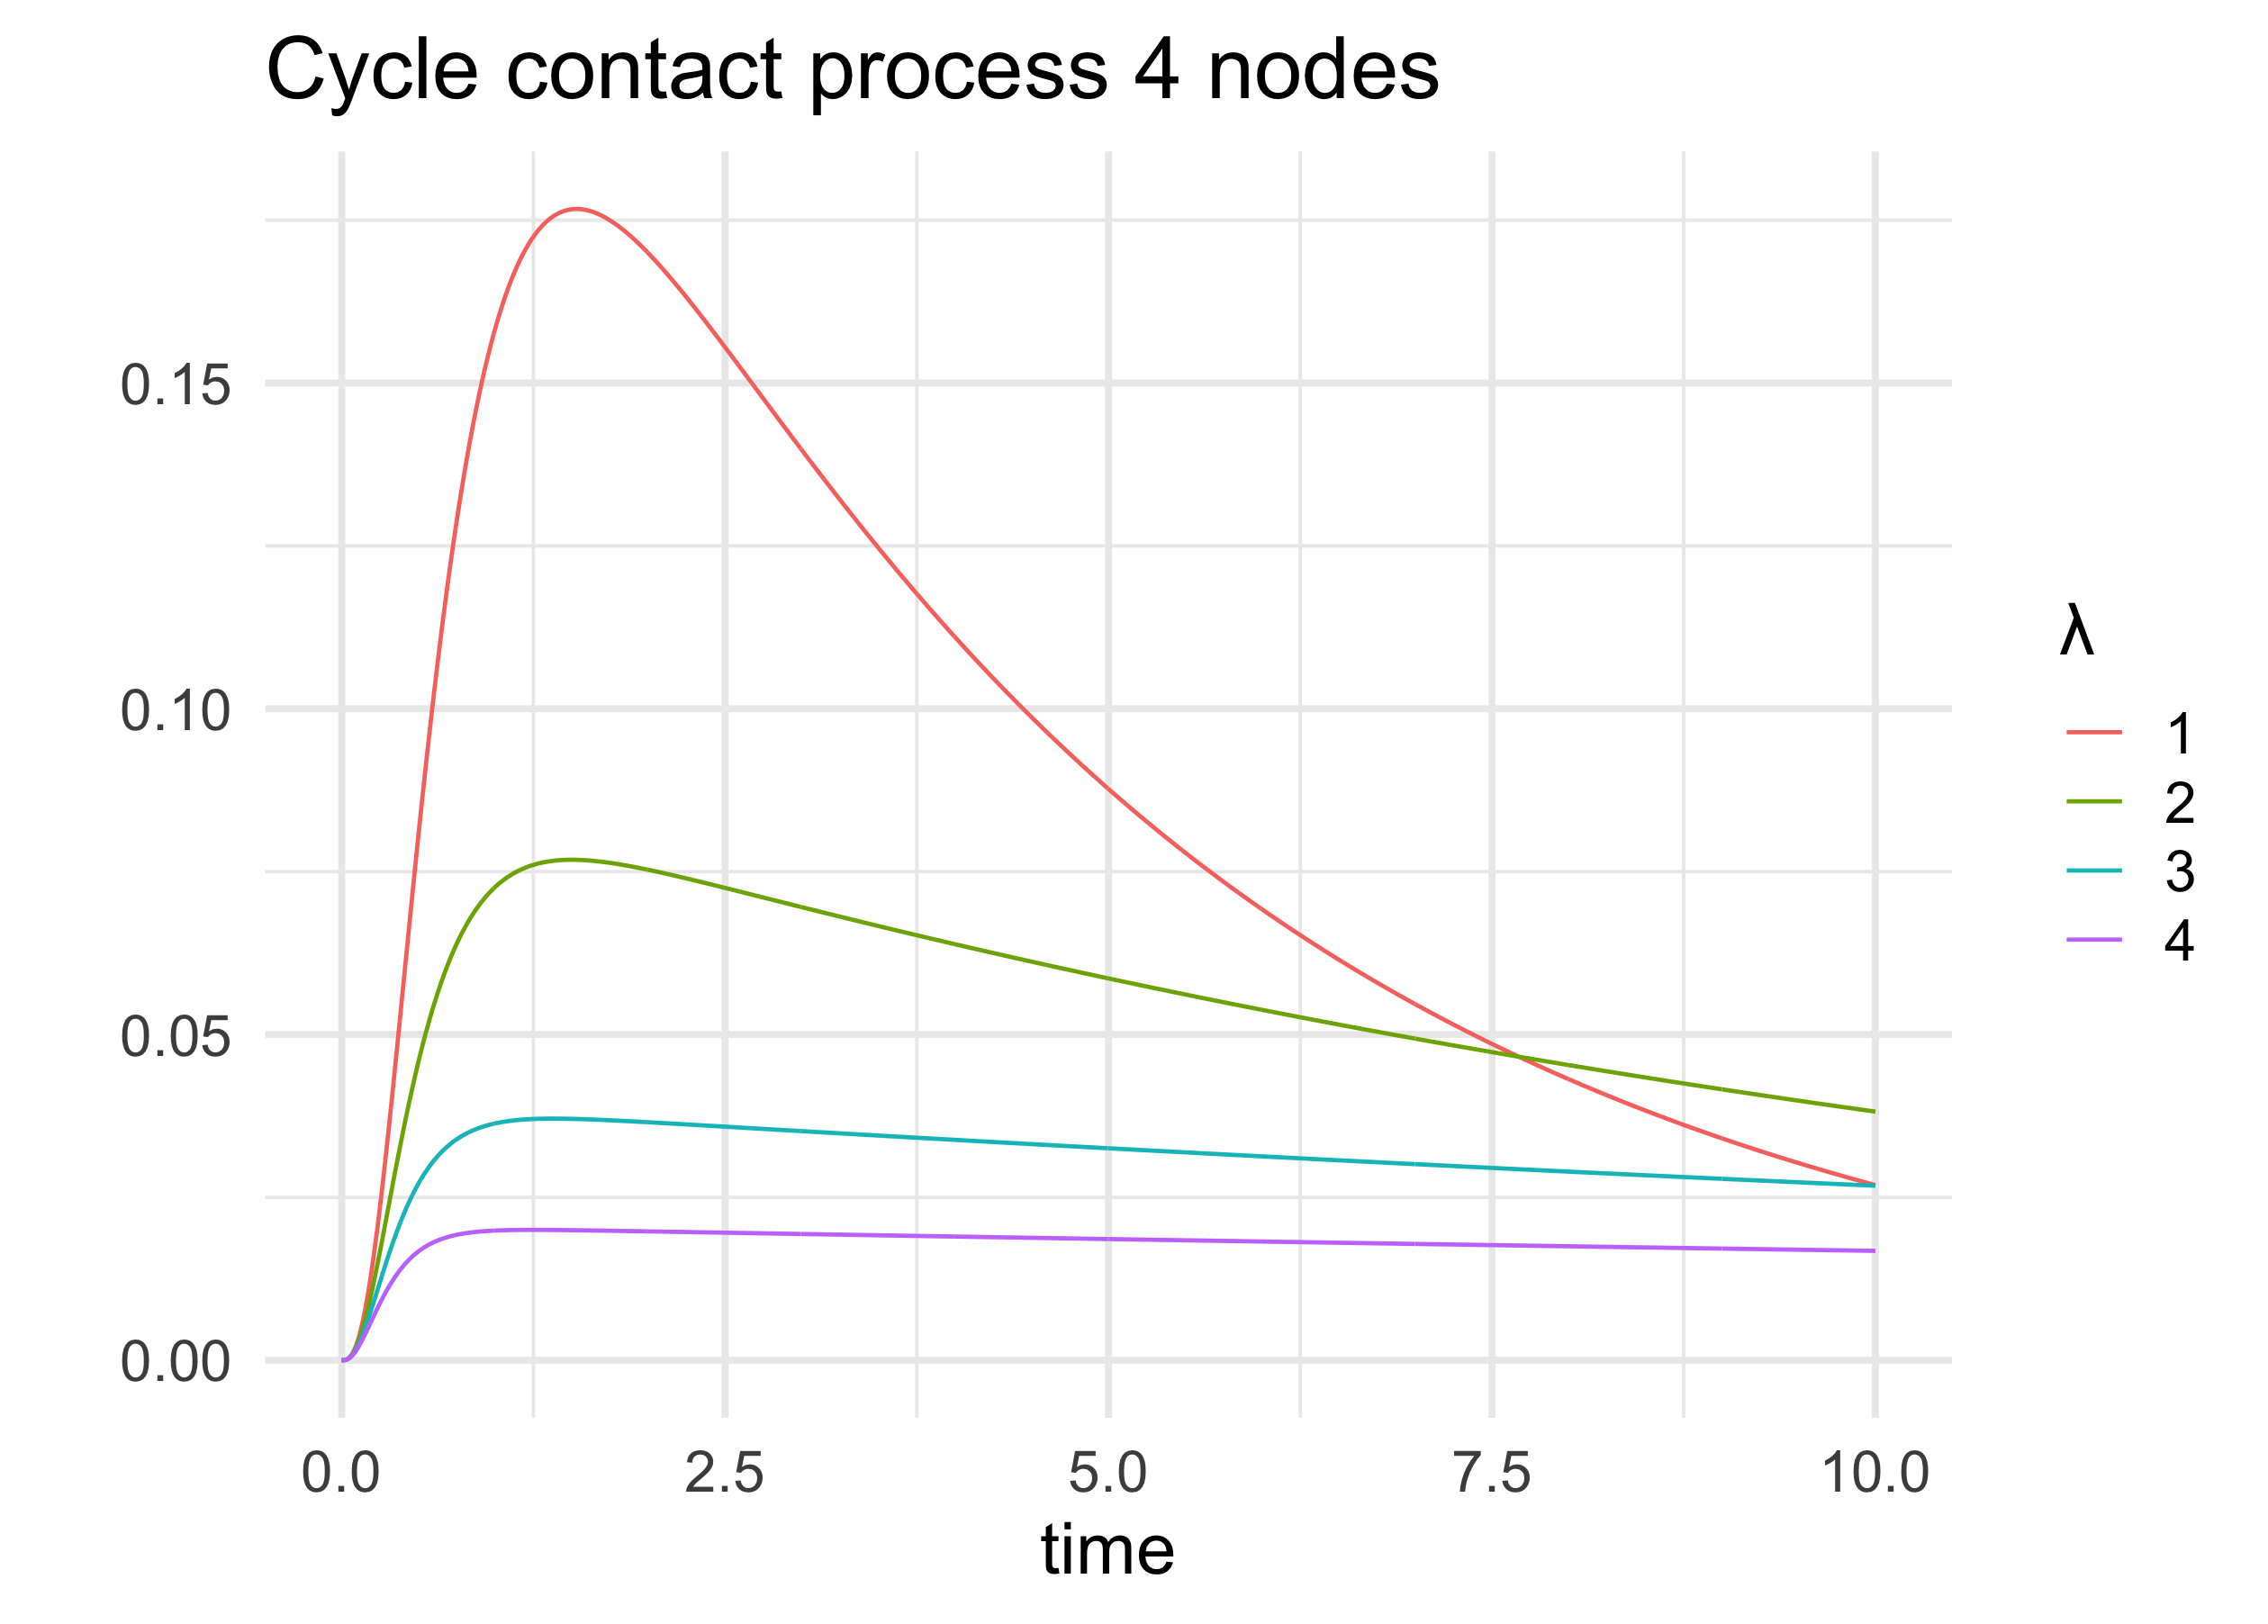
\includegraphics[width=.80\textwidth]{figures/cycle_4_contact_phase_densities.png}
   \caption{Density functions for $\tau_{S_4}$ for $\lambda = 1, 2, 3, 4$ on the four node contact process on a cycle}
  \label{fig:contact_4_cycle_phase_densities}
\end{figure}

\subsection{Finite contact process on 1D lattice}

Now we look at a contact process on a finite subset of a 1-dimensional lattice.
That is, two nodes will have exactly one edge while the rest will have two edges.
This is in contrast to the cycle which has exactly two edges for each node.
The two node contact process on the lattice is identical to the complete graph.

\subsubsection{Three node contact process \texorpdfstring{$L_3$}{L3}}
We can project the three node contact process with two edges onto a new Markov chain by Theorem \ref{thm:mc_projection} by associating states 110 and 011 as well as 100 and 001.
For the three node contact process with two edges, we have a transition graph shown in Figure \ref{fig:three_node_contact_lattice_states}.

\begin{figure}[H]
    \centering
   %\begin{tikzpicture}[auto, node distance=2cm, every loop/.style={-Triangle}, thick,main node/.style={circle,draw}]
  \begin{tikzpicture}[start chain = going right,
   -Triangle, every loop/.append style = {-Triangle}]
   \node[state, on chain]  (111) {111};
   \node[state, on chain]  (110) [above right of=111, yshift = 4mm]  {110};
   \node[state, on chain]  (101) [below right of=111, yshift = -4mm]  {101};

   \node[state, on chain]  (010) [right of=110, xshift=3mm]  {010};
   \node[state, on chain]  (100) [right of=101, xshift=3mm]  {100};

   \node[state, on chain]  (000) [below right of=010]  {000};


   \draw (111) edge [bend left] node[yshift=3.5mm, xshift=-1mm]{$2$} (110);
   \draw (110) edge [] node[yshift=-2mm, xshift=1.5mm]{$\lambda$} (111);

   \draw (111) edge [bend right] node[yshift=-3mm]{$1$} (101);
   \draw (101) edge [] node[yshift=1.5mm, xshift = 2mm]{$2\lambda$} (111);

   \draw (110) edge [bend left] node[yshift=3mm]{$1$} (010);
   \draw (010) edge [] node[yshift=-2mm, xshift=1.5mm]{$2 \lambda$} (110);

   \draw (101) edge [] node[yshift=-3mm]{$2$} (100);

   \draw (110) edge [] node[yshift=3mm]{$1$} (100);
   \draw (100) edge [bend left] node[yshift=3mm]{$\lambda$} (110);

  \draw (010) edge [] node[yshift=3mm]{$1$} (000);
  \draw (100) edge [] node[yshift=-3mm]{$1$} (000);

\end{tikzpicture}
    \caption{Three node contact process on 1D lattice projected rates between each states}
    \label{fig:three_node_contact_lattice_states}
\end{figure}

\begin{equation}
Q_{L_3} =
\begin{blockarray}{ccccccc}
    & 111 & 110 & 101 & 100 & 010 & 000\\
    \begin{block}{c|cccccc}
    \cline{2-7}
    111 & -3 & 2 & 1 & 0 & 0 & 0\\
    110 & \lambda & -(\lambda + 2) & 0 & 1 & 1 & 0\\
    101 & \lambda & 0 & -(\lambda + 1) & 1 & 0 & 0\\
    100 & 0 & \lambda & 0 & -(\lambda + 1) & 0 & 1\\
    010 & 0 & 2\lambda & 0 & 0 & -(2\lambda + 1) & 1\\
    000 & 0 & 0 & 0 & 0 & 0 & 0\\
    \end{block}
\end{blockarray}
\end{equation}

\subsubsection{Phase-type Distribution}

In Figure \ref{fig:lattice_3_contact_phase_densities} we plot the density functions for $\tau_{L_3}$ for $\lambda = 1, 2, 3, 4$ on the four node contact process on a cycle.

\begin{figure}[H]
  \centering
    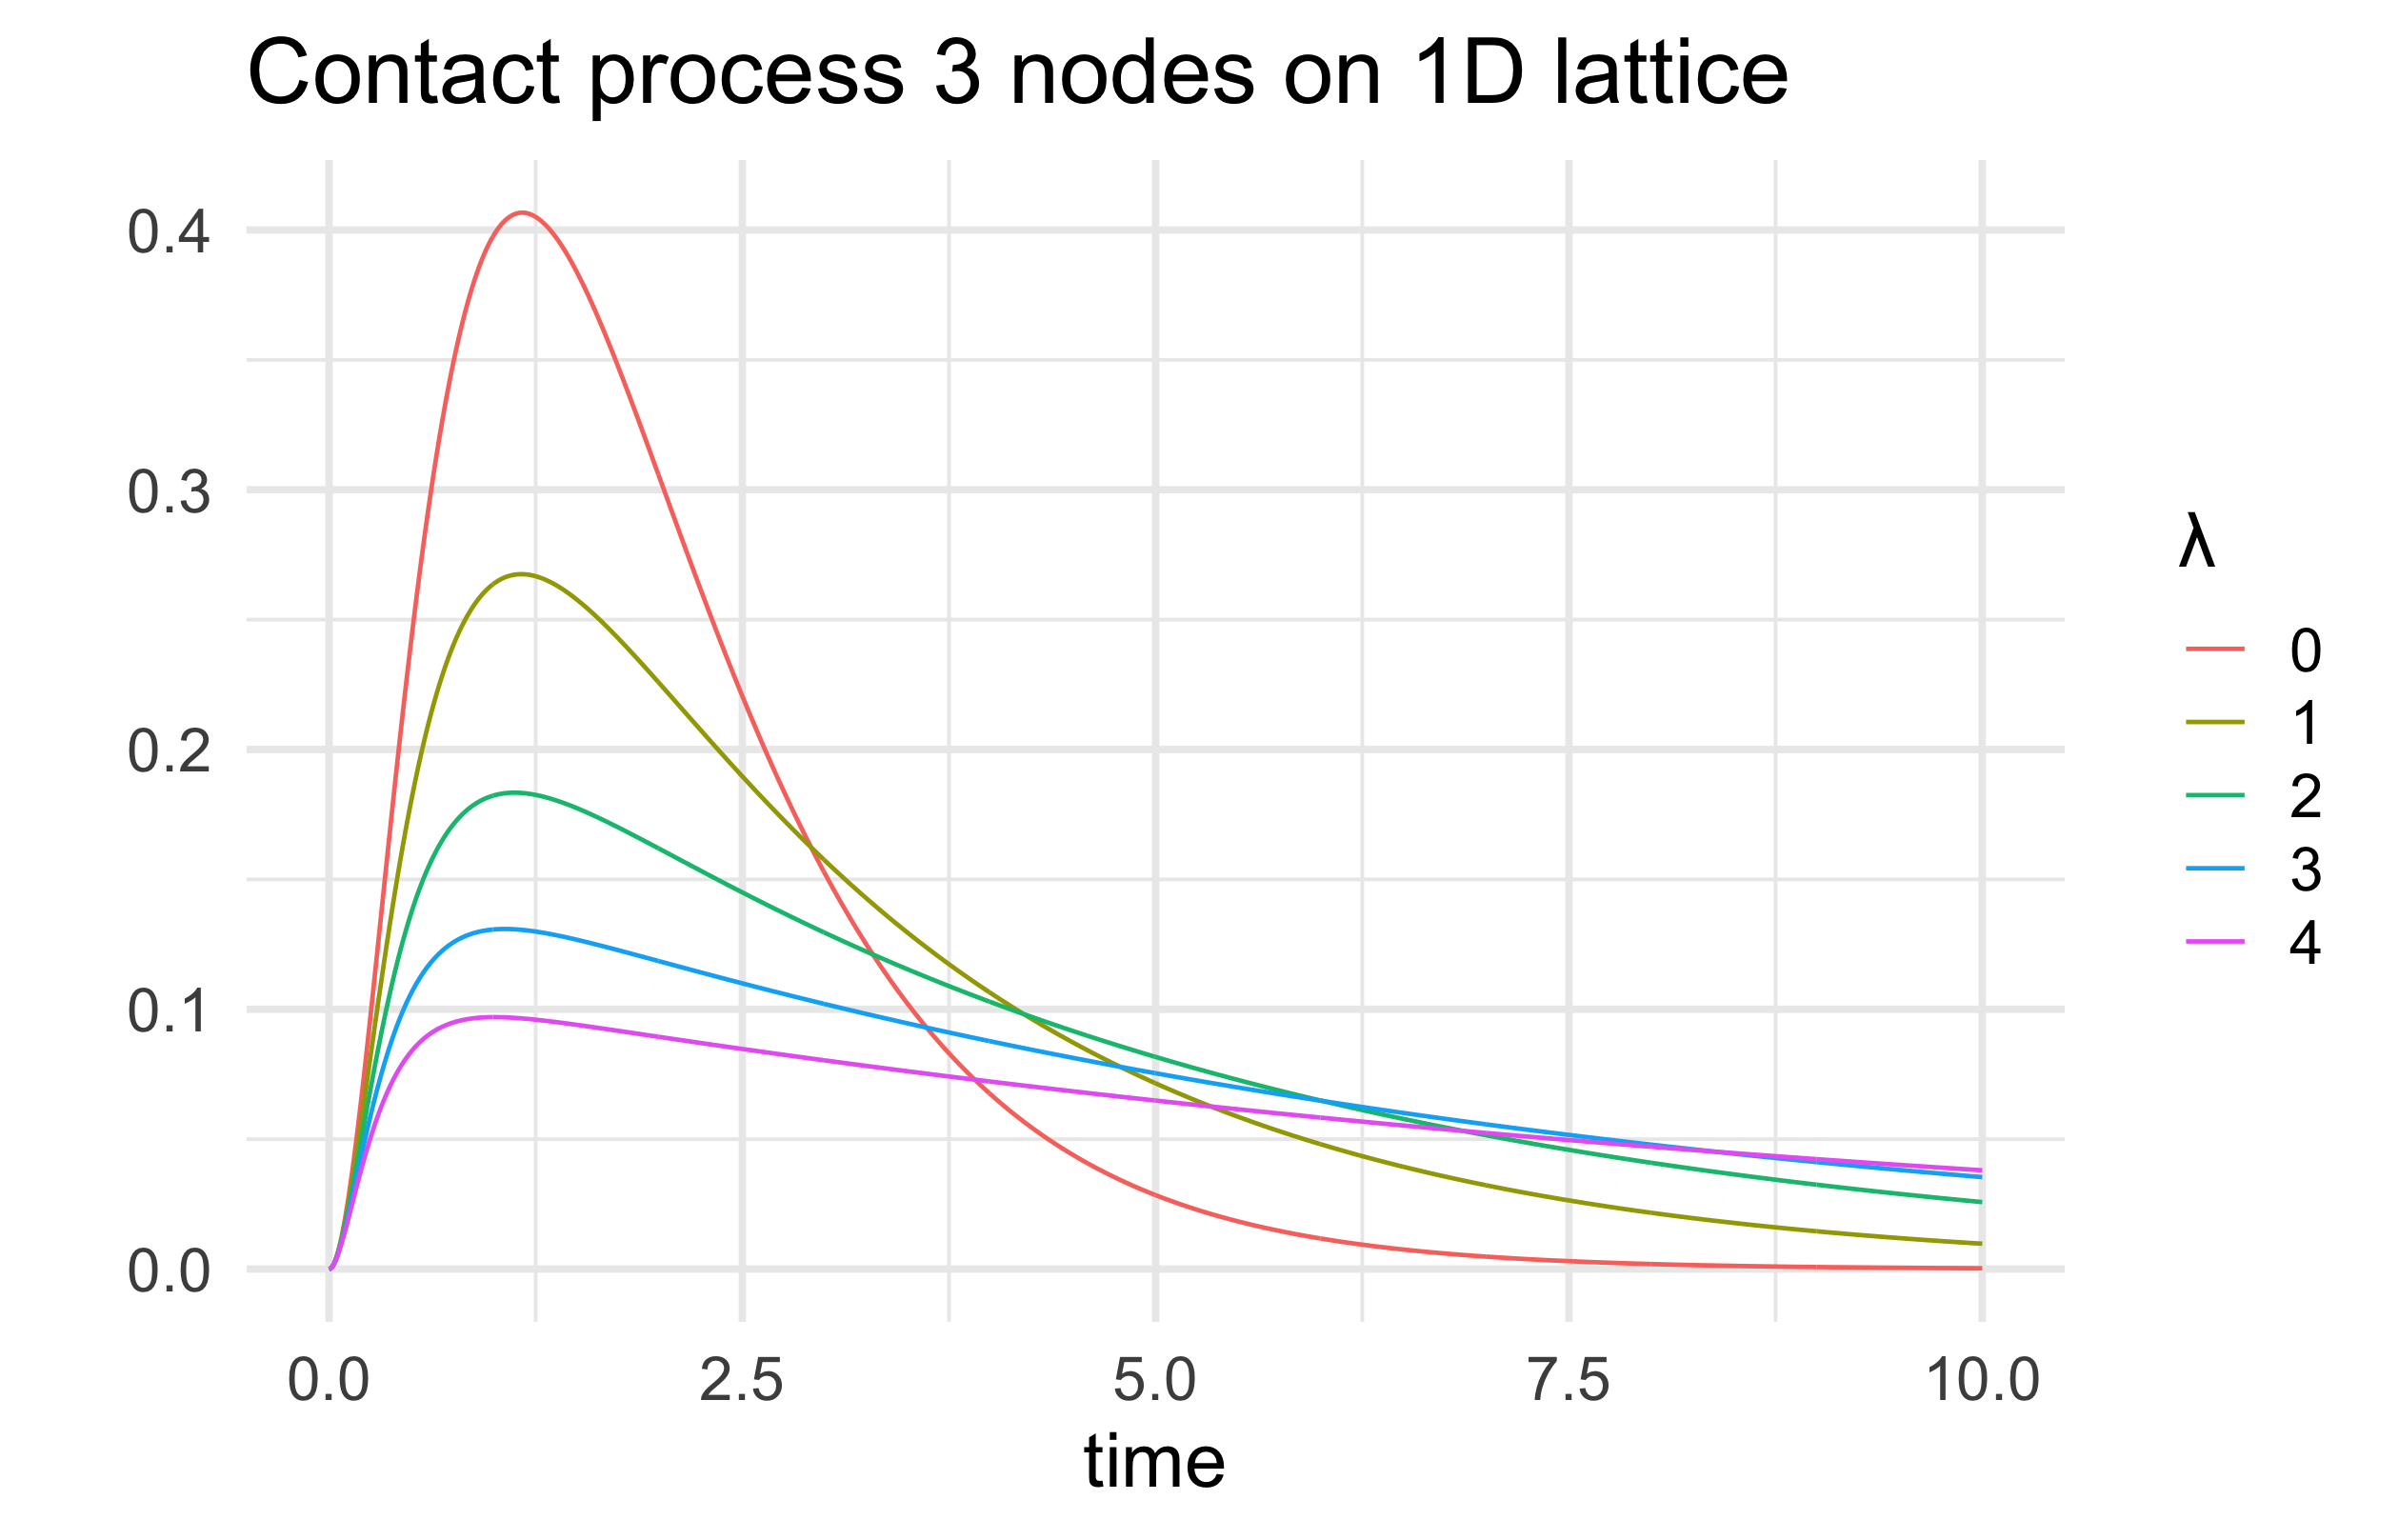
\includegraphics[width=.80\textwidth]{figures/lattice_3_contact_phase_densities.png}
   \caption{Density functions for $\tau_{L_3}$ for $\lambda = 1, 2, 3, 4$ on the four node contact process on a cycle}
  \label{fig:lattice_3_contact_phase_densities}
\end{figure}

\subsection{Comparison of Phase-type distributions for \texorpdfstring{$C_2$}{C2}, \texorpdfstring{$C_3$}{C3}, \texorpdfstring{$L_3$}{L3}, and \texorpdfstring{$S_4$}{S4}}

All of the graph configurations are identical when we have two nodes.
Also, $S_3$ is the same as $C_3$.
In Figure \ref{fig:ev_phase_comparison_3.png} we compare of expected values of $\tau_{C_2}$, $\tau_{C_3}$, and $\tau_{L_3}$.
Since $\tau_{S_4}$ is much larger than $\tau_{C_2}$, $\tau_{C_3}$, and $\tau_{L_3}$ we include it separately in Figure \ref{fig:ev_phase_comparison_4.png}.

\begin{figure}[H]
  \centering
    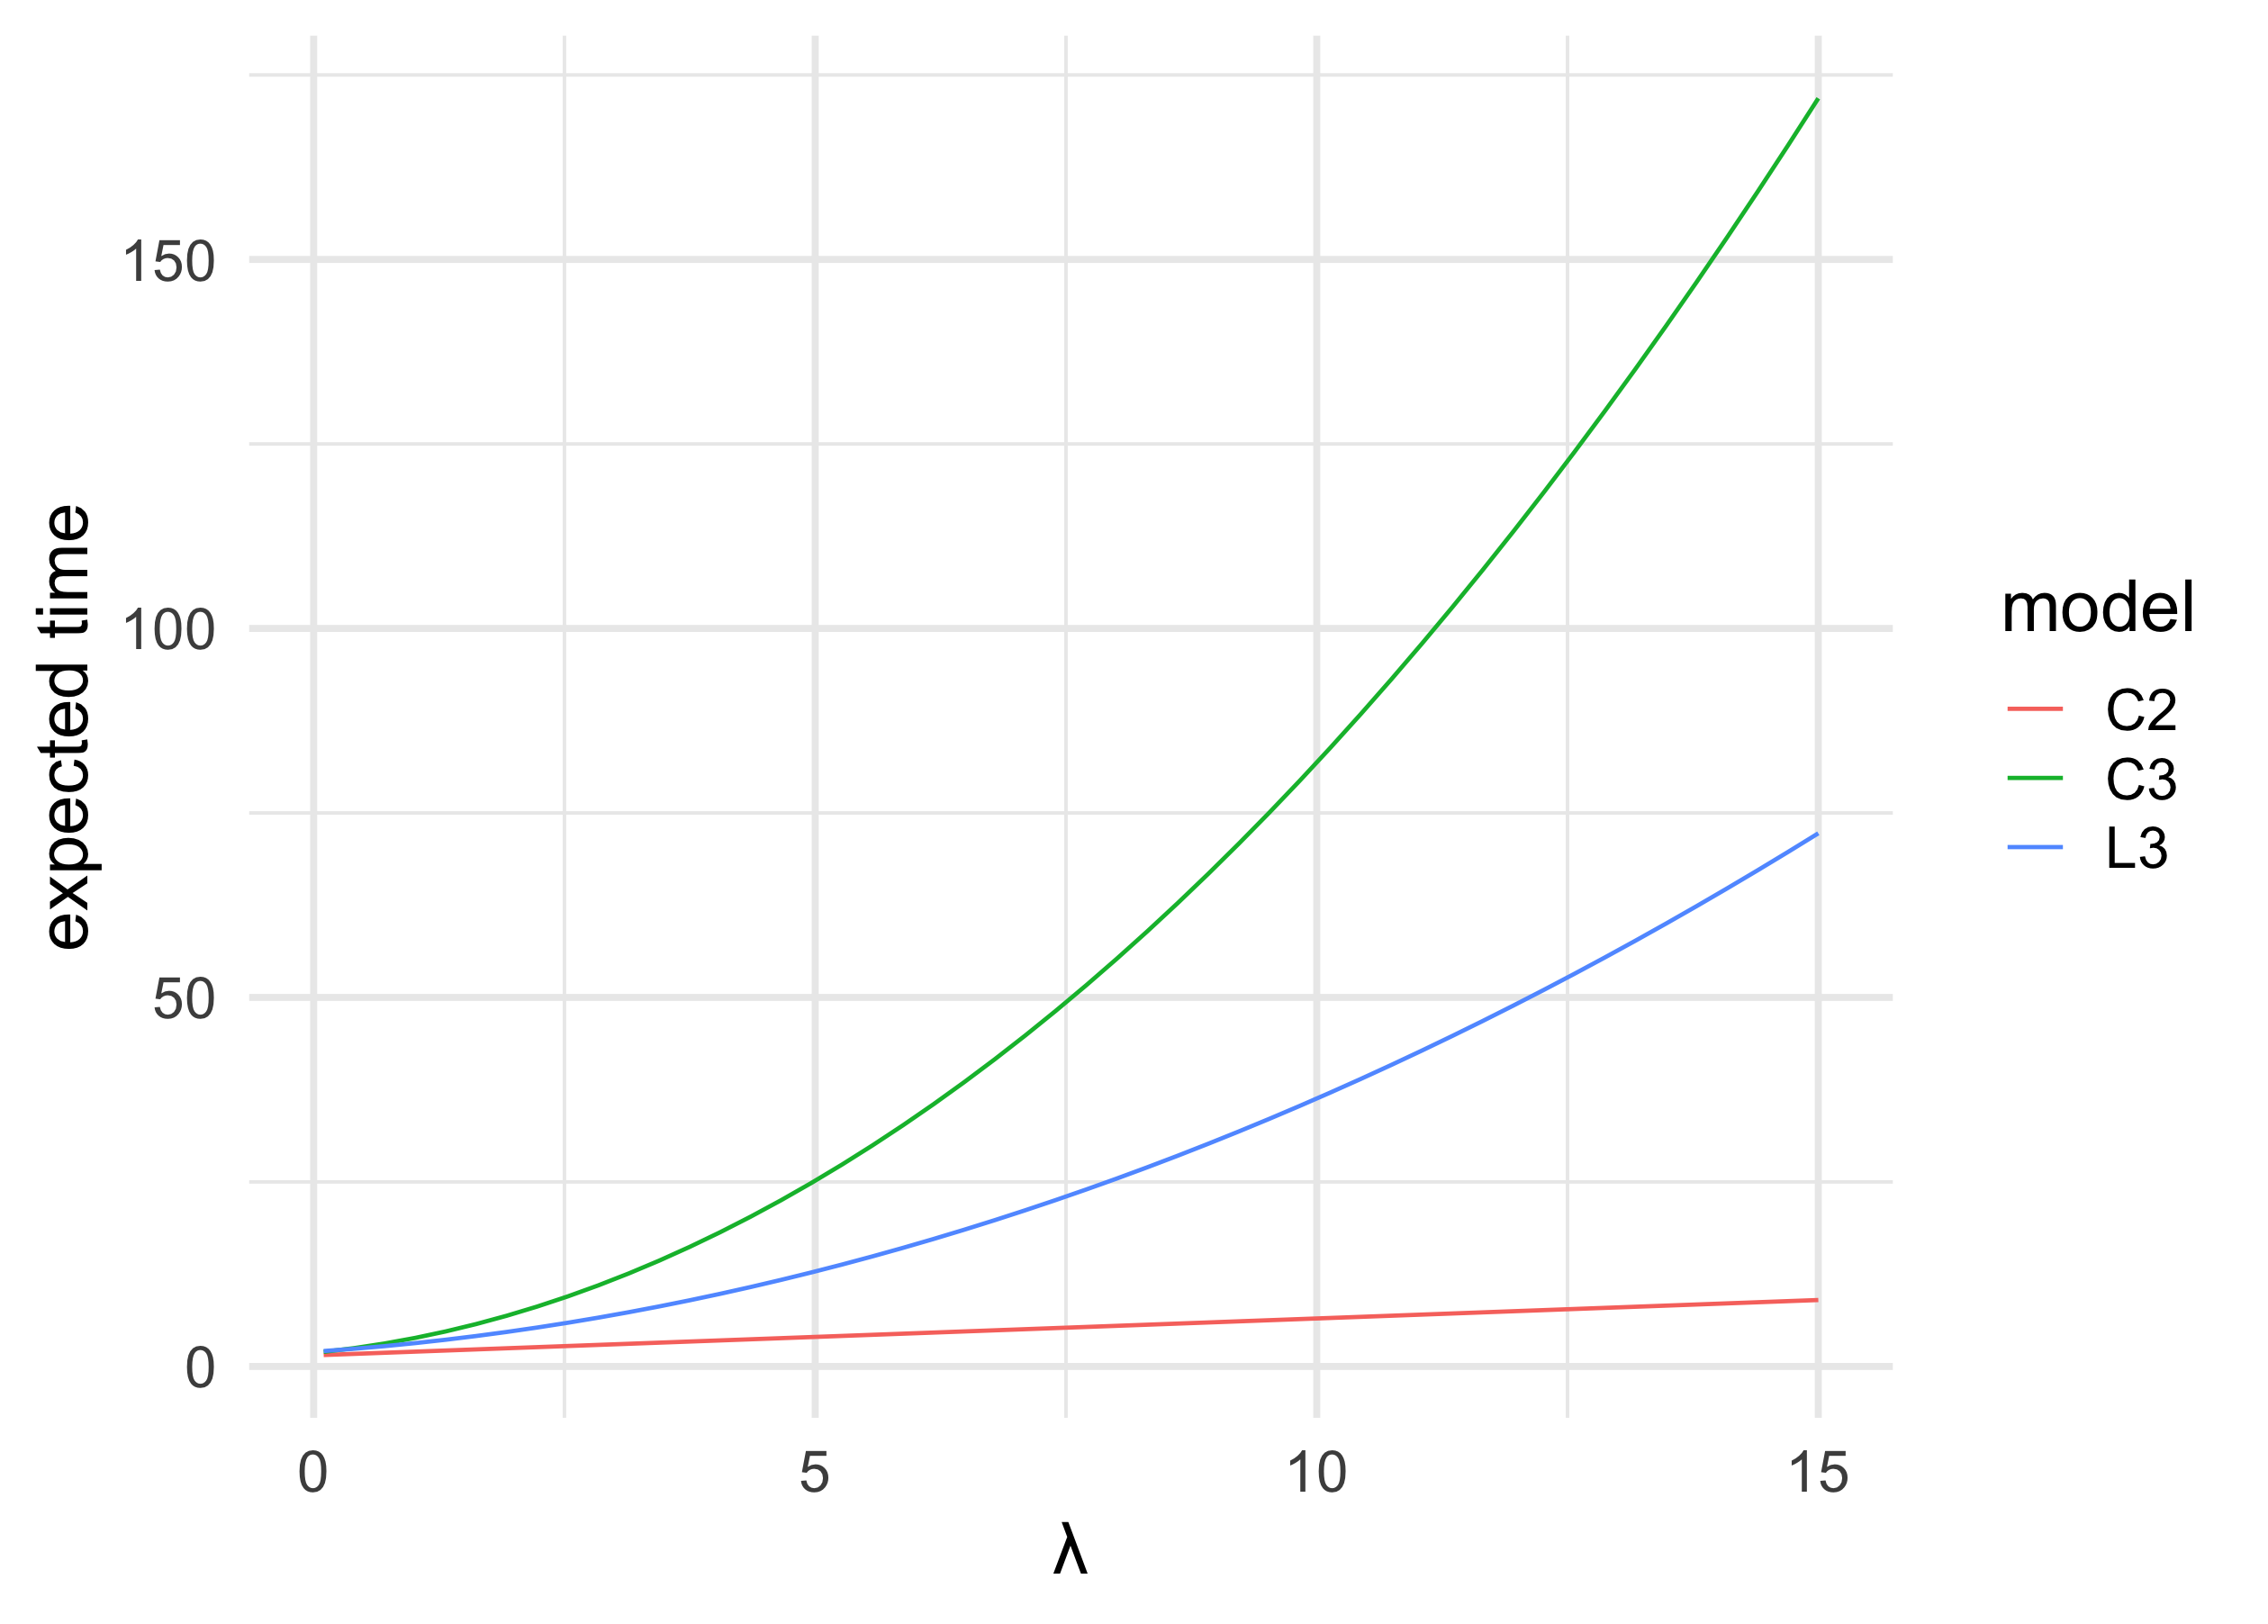
\includegraphics[width=.80\textwidth]{figures/ev_phase_comparison_3.png}
   \caption{Comparison of expected values of $\tau_{C_2}$, $\tau_{C_3}$, and $\tau_{L_3}$}
  \label{fig:ev_phase_comparison_3.png}
\end{figure}

\begin{figure}[H]
  \centering
    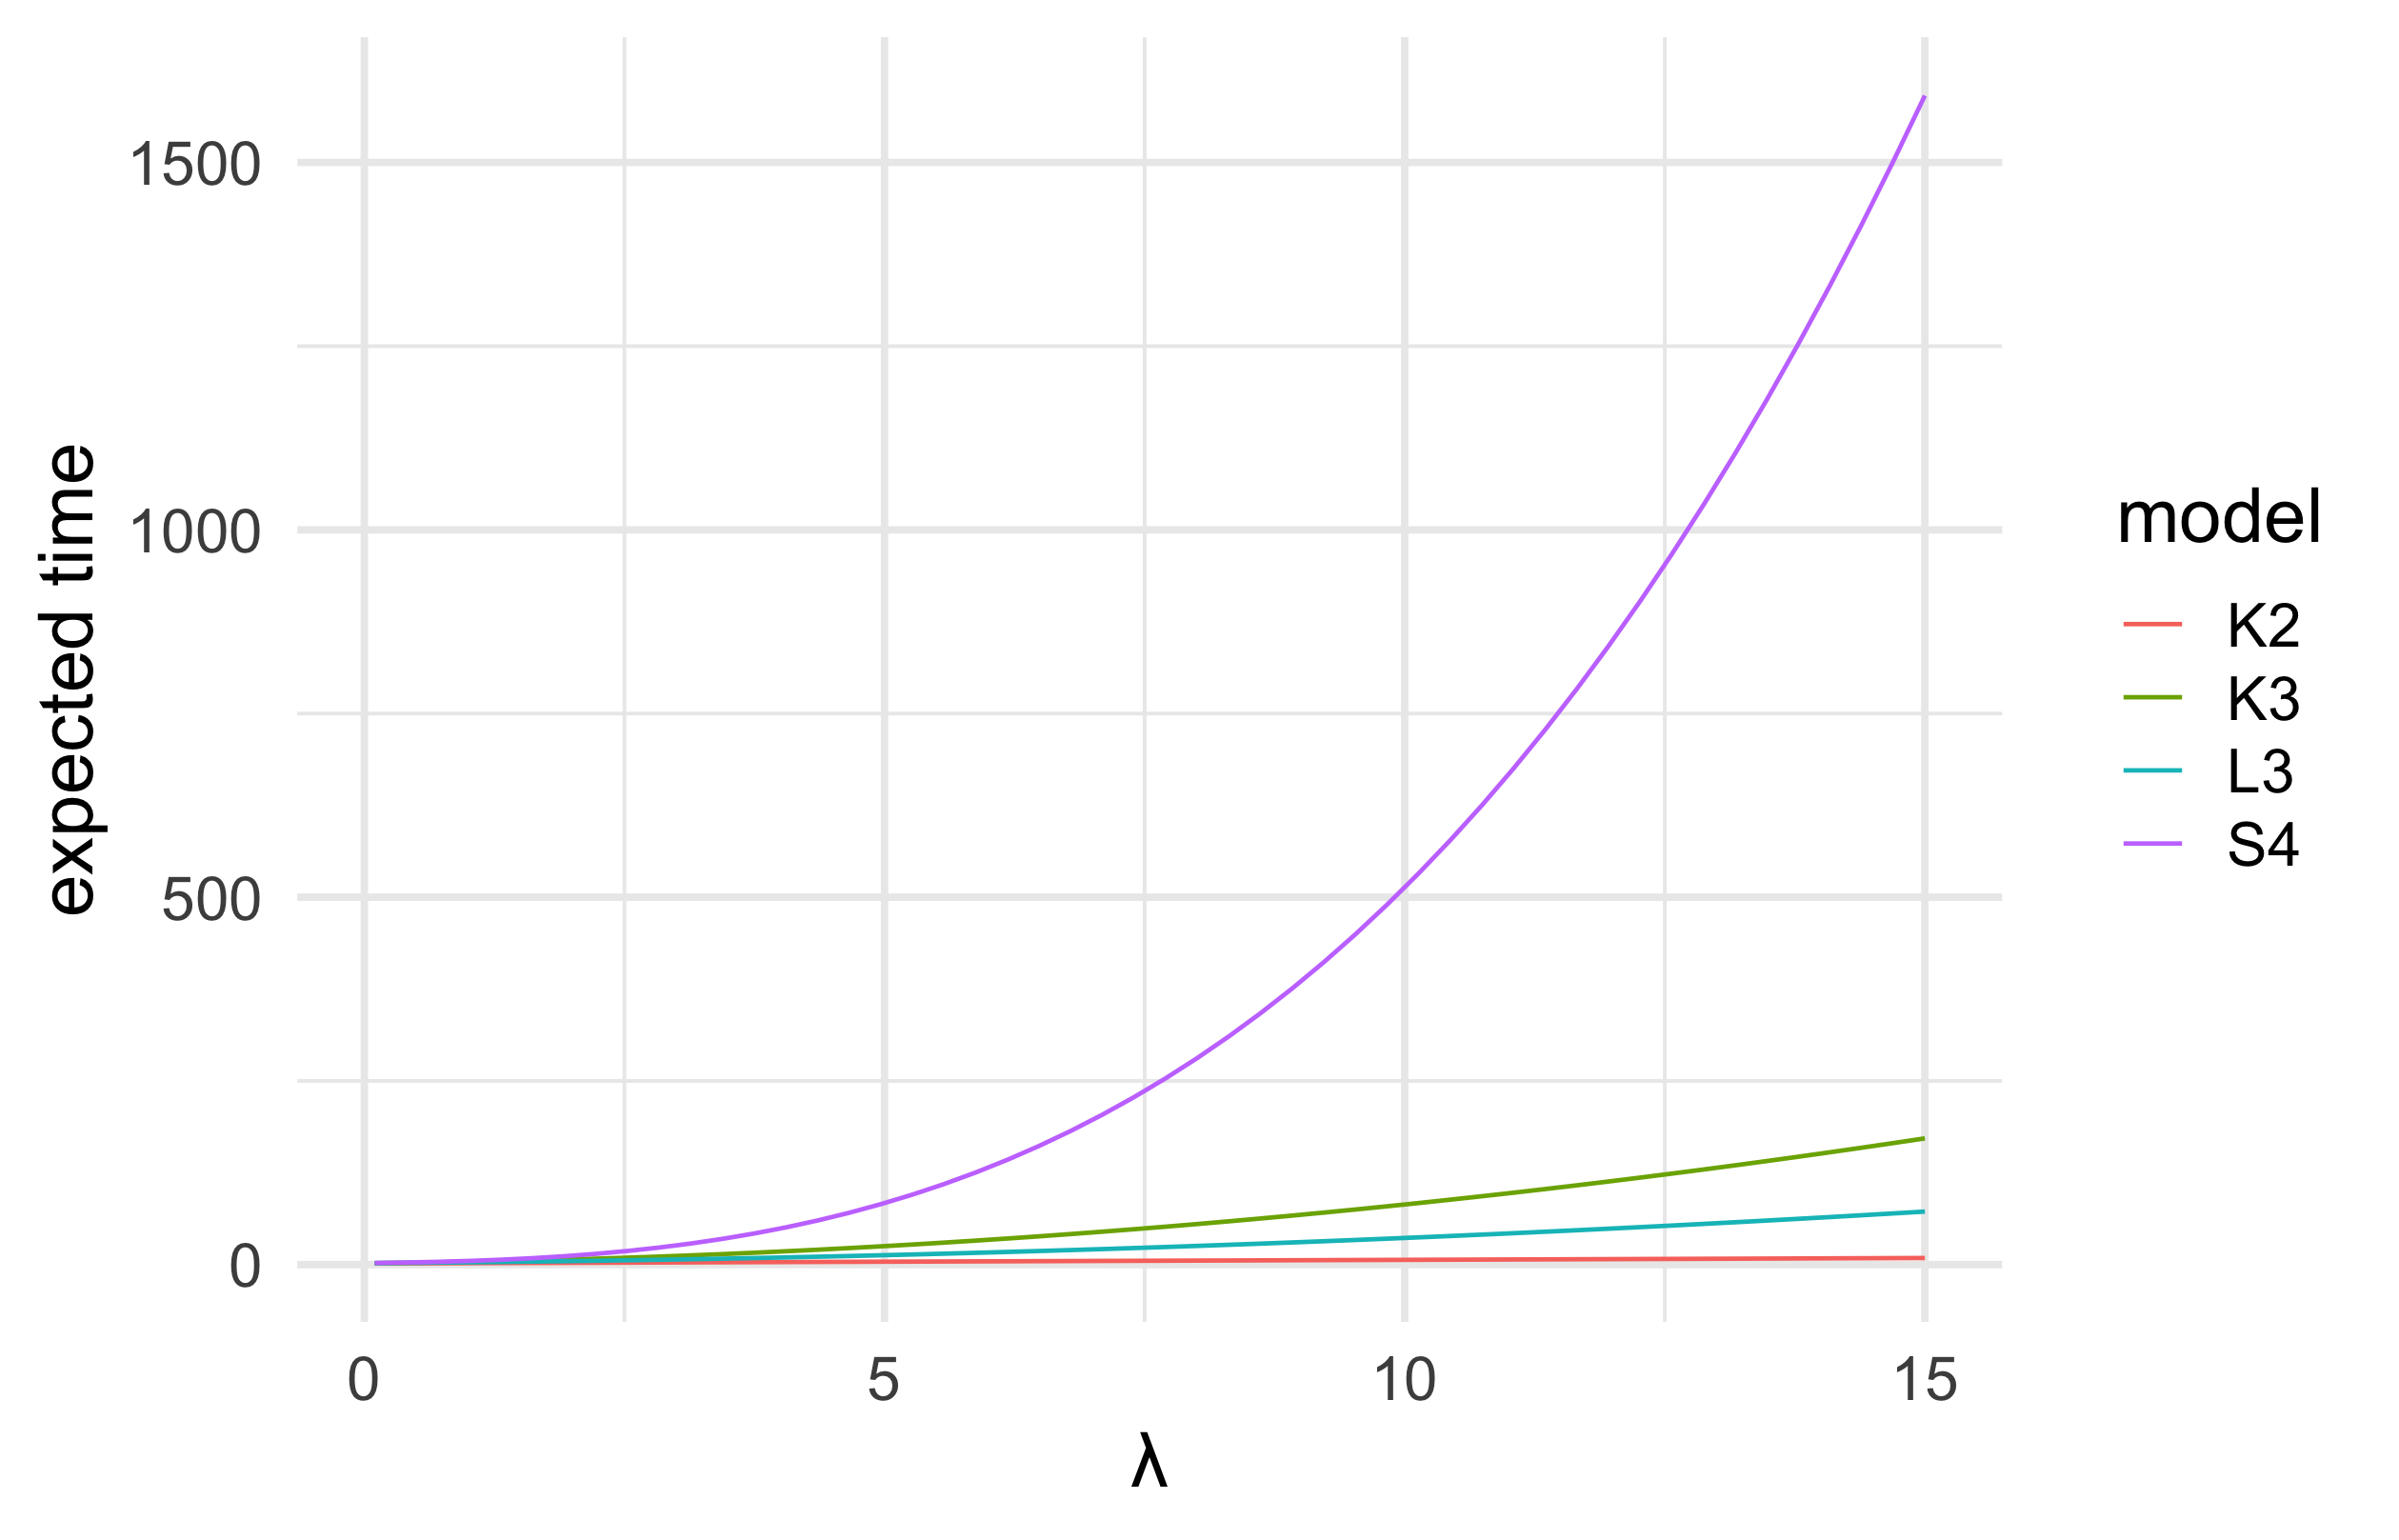
\includegraphics[width=.80\textwidth]{figures/ev_phase_comparison_4.png}
   \caption{Comparison of expected values of $\tau_{C_2}$, $\tau_{C_3}$, $\tau_{L_3}$, and $\tau_{S_4}$}
  \label{fig:ev_phase_comparison_4.png}
\end{figure}